\documentclass[a4paper,12pt]{article}

\usepackage{fontspec}
\usepackage[vietnamese,provide=*]{babel}
\usepackage{amsmath,amssymb}
\usepackage{graphicx}
\usepackage{booktabs}
\usepackage{adjustbox}
\usepackage{xcolor}
\usepackage{tikz}
\usetikzlibrary{positioning,fit,arrows.meta,calc}
\tikzset{
  blk/.style={draw, rounded corners=2pt, minimum height=1.2cm, minimum width=1.6cm,
              align=center, font=\scriptsize, inner sep=1.5pt},
  inp/.style={blk, fill=gray!15},
  flt/.style={blk, fill=gray!15},
  cnv/.style={blk, fill=blue!15},
  pol/.style={blk, fill=orange!20},
  lin/.style={blk, fill=green!15},
  rowlbl/.style={align=center, font=\small\bfseries, text width=1.9cm},
  arr/.style={-{Latex[length=1.8mm]}, thick}
}
\usepackage{minted}
\usepackage[top=2.5cm, bottom=2.0cm, left=3.0cm, right=2.0cm]{geometry}
\usepackage{setspace}\onehalfspacing
\usepackage[hidelinks]{hyperref}

\DeclareMathOperator{\softmax}{softmax}

\setmainfont{Latin Modern Roman}
\setsansfont{Latin Modern Sans}
\setmonofont{Latin Modern Mono}

% TODO: remove when done
\newcommand{\todo}[1]{\textcolor{red}{[TODO: #1]}}
\newcommand{\figph}[2]{\fbox{\parbox[c][#1][c]{0.92\linewidth}{\centering\textcolor{gray}{[Chỗ chèn hình: #2]}}}}

\begin{document}
\begin{titlepage}
    \begin{center}
        ĐẠI HỌC QUỐC GIA THÀNH PHỐ HỒ CHÍ MINH \\
        TRƯỜNG ĐẠI HỌC BÁCH KHOA \\
        KHOA KHOA HỌC VÀ KỸ THUẬT MÁY TÍNH
    \end{center}

    \vspace{1cm}

    \begin{center}
        
\includegraphics[width=3cm]{images/logo.png}
    \end{center}

    \vspace{1cm}

    \begin{center}
        \begin{tabular}{c}
            \multicolumn{1}{c}{\textbf{{\Large HỌC SÂU VÀ ỨNG DỤNG}}}              \\
            \multicolumn{1}{c}{\textbf{{\Large TRONG THỊ GIÁC MÁY TÍNH (CO5085)}}} \\
            ~~                                                                     \\
            \hline
            \\ \\
            \textbf{{\huge Báo cáo Bài tập E1--E3}}                                \\
            \\ \\
            \hline
        \end{tabular}
    \end{center}

    \vspace{1.5cm}

    \begin{table}[h]
        \begin{tabular}{rrll}
            \hspace{5.5 cm} & GVHD:      & \multicolumn{2}{l}{TS.\ Lê Thành Sách}              \\
                            &            & \multicolumn{2}{l}{TS.\ Nguyễn Quốc Minh}           \\
                            & Sinh viên: & Lê Hữu Trọng                              & 2470578 \\
                            &            & Huỳnh Văn Tâm Thiện                       & 2470094 \\
        \end{tabular}
    \end{table}

    \vspace{1.5cm}

    \begin{center}
        {\footnotesize THÀNH PHỐ HỒ CHÍ MINH, THÁNG 10/2026}
    \end{center}
\end{titlepage}
\newpage
\tableofcontents
\newpage

\section{Giới thiệu}
\label{sec:intro}

Báo cáo này khảo sát và so sánh hiệu suất của các mô hình học sâu thông qua ba bài tập E1--E3. Để đối chiếu trực tiếp các phương pháp, chúng tôi dùng chung một tập ảnh nhỏ cho cả ba bài. Toàn bộ mã nguồn, tài liệu và kết quả chi tiết của các thực nghiệm được công khai tại các địa chỉ sau:
\begin{itemize}
    \item GitHub Repository: \url{https://github.com/tronglh241/co5085_dl4cv}
    \item GitHub Pages: \url{https://tronglh241.github.io/co5085_dl4cv}
\end{itemize}

Nội dung chính của các bài tập được triển khai như sau:
\begin{itemize}
    \item \textbf{Bài E1 (Mục~\ref{sec:e1}):} So sánh ba bộ phân loại cơ bản gồm Softmax, Multilayer Perceptron (MLP) và Convolutional Neural Network (CNN), được đánh giá trong cả hai trường hợp có và không có kỹ thuật tăng cường dữ liệu.
    \item \textbf{Bài E2 (Mục~\ref{sec:e2}):} Xây dựng bộ phân loại dựa trên cơ chế Multi-Head Self-Attention (MSA), trong đó, chúng tôi hiện thực MSA từ đầu để đối chiếu với module sẵn có của PyTorch, đồng thời khảo sát các phương pháp chuyển đổi ảnh thành chuỗi token khác nhau.
    \item \textbf{Bài E3 (Mục~\ref{sec:e3}):} Xem xét ảnh dưới góc độ dữ liệu chuỗi để huấn luyện các mô hình hồi quy Long Short-Term Memory (LSTM) và Gated Recurrent Unit (GRU), sau đó so sánh kết quả với các mô hình không hồi quy đã khảo sát ở bài E1.
\end{itemize}

Mục tiêu của báo cáo không dừng lại ở việc liệt kê accuracy của từng mô hình, mà tập trung giải thích nguyên nhân dẫn đến sự khác biệt về hiệu suất thông qua số lượng tham số, đường cong học và phân tích chi tiết các trường hợp phân loại sai.

Phần còn lại của báo cáo được tổ chức như sau. Mục~\ref{sec:data} mô tả dữ liệu, phương pháp tiền xử lý và đánh giá dùng chung cho cả ba bài. Các Mục~\ref{sec:e1}, \ref{sec:e2} và \ref{sec:e3} lần lượt trình bày bài E1, E2 và E3, mỗi mục gồm mô hình, thiết lập huấn luyện riêng, kết quả và thảo luận. Mục~\ref{sec:summary} so sánh kết quả giữa ba bài, sau đó là phần kết luận và các phụ lục.

\section{Dữ liệu và phương pháp đánh giá}
\label{sec:data}

\subsection{Tập dữ liệu và cách chia}
\label{sec:split}

Trong báo cáo này, chúng tôi sử dụng MNIST \cite{lecun1998gradient}, tập dữ liệu chuẩn gồm các ảnh chữ số viết tay dạng ảnh xám với kích thước $28\times28$ điểm ảnh, gồm 10 lớp từ 0 đến 9. Bộ dữ liệu gốc bao gồm $60\,000$ ảnh huấn luyện và $10\,000$ ảnh kiểm thử chính thức. Việc lựa chọn MNIST dựa trên ba lý do chính:
\begin{itemize}
    \item \textbf{Tốc độ huấn luyện:} Kích thước ảnh nhỏ và chỉ có một kênh màu giúp rút ngắn thời gian huấn luyện, tạo điều kiện thử nghiệm nhiều biến thể cấu trúc.
    \item \textbf{Tính chuẩn hóa:} Là một bộ dữ liệu tham chiếu phổ biến, MNIST giúp dễ dàng đối chiếu, so sánh kết quả của các mô hình.
    \item \textbf{Sự cân bằng dữ liệu:} Các lớp trong MNIST có phân bố số lượng tương đối đồng đều, giúp độ đo accuracy phản ánh trung thực hiệu suất tổng thể của mô hình mà không bị ảnh hưởng bởi hiện tượng mất cân bằng lớp.
\end{itemize}

Từ $60\,000$ ảnh huấn luyện gốc, chúng tôi tách thành $50\,000$ ảnh cho tập huấn luyện và $10\,000$ ảnh cho tập kiểm định theo phương pháp phân tầng (stratified splitting) để duy trì tỷ lệ các lớp đồng đều giữa các tập. Quá trình chia dữ liệu được thực hiện duy nhất một lần nhằm đảm bảo mọi mô hình trong các bài tập E1, E2 và E3 đều được huấn luyện và đánh giá trên cùng một tập dữ liệu. Tập kiểm thử chính thức được giữ nguyên hoàn toàn tách biệt khỏi quá trình huấn luyện. Số lượng ảnh của từng lớp được thể hiện trong Bảng~\ref{tab:class-dist}, phân bố của các lớp được thể hiện trong Hình~\ref{fig:class-balance}, trong khi Hình~\ref{fig:samples} minh họa một số mẫu dữ liệu từ các lớp khác nhau.

\begin{figure}[t]
    \centering
    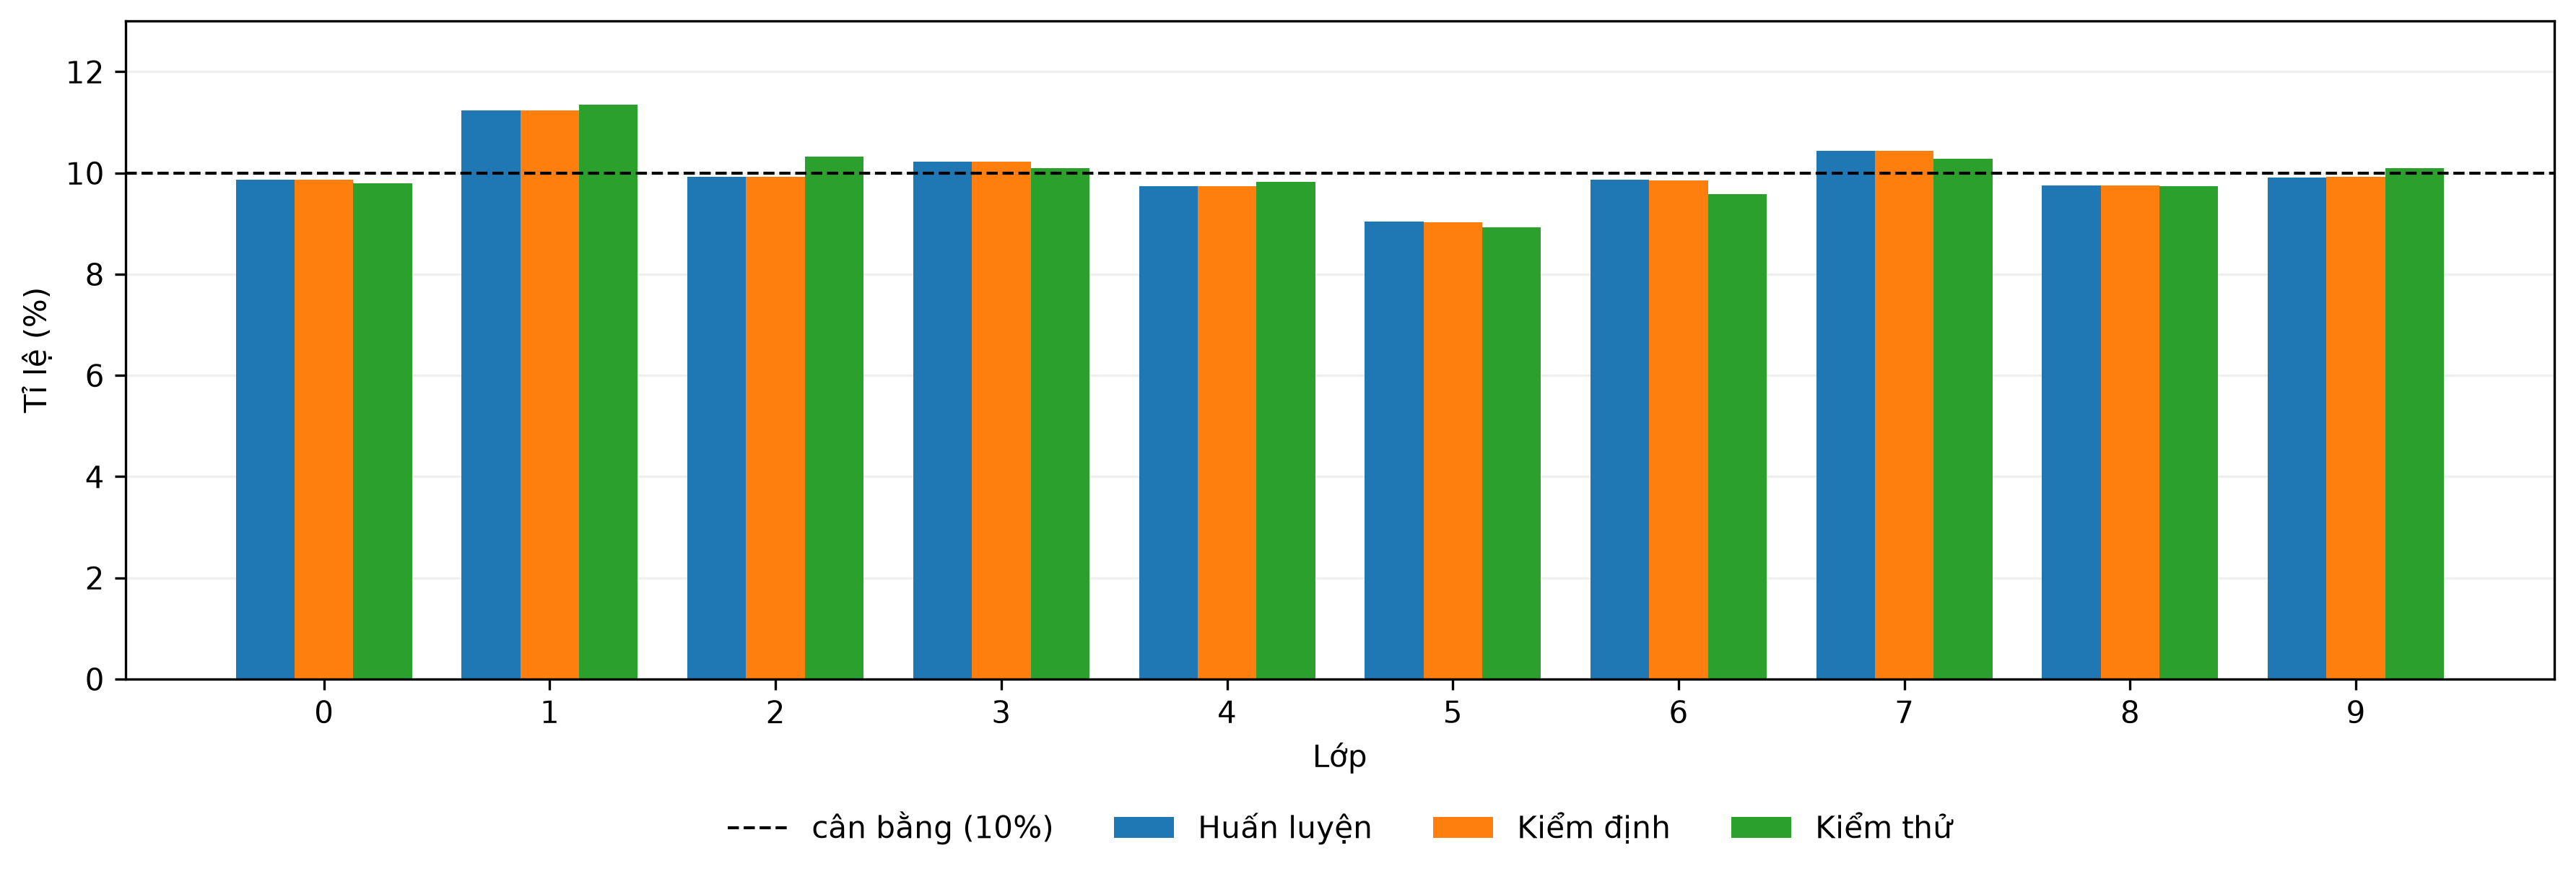
\includegraphics[width=\textwidth]{../docs/assets/shared/class_balance.png}
    \caption{Biểu đồ thể hiện sự phân bố mẫu dữ liệu giữa các lớp trong tập dữ liệu MNIST, minh họa tính cân bằng dữ liệu.}
    \label{fig:class-balance}
\end{figure}

\begin{table}[t]
    \centering
    \caption{Số lượng ảnh của từng lớp trong các tập dữ liệu.}
    \label{tab:class-dist}
    \small
    \begin{tabular}{lrrr}
        \toprule
        Lớp  & Huấn luyện & Kiểm định & Kiểm thử \\
        \midrule
        0    & 4\,936     & 987       & 980      \\
        1    & 5\,618     & 1\,124    & 1\,135   \\
        2    & 4\,965     & 993       & 1\,032   \\
        3    & 5\,109     & 1\,022    & 1\,010   \\
        4    & 4\,868     & 974       & 982      \\
        5    & 4\,518     & 903       & 892      \\
        6    & 4\,932     & 986       & 958      \\
        7    & 5\,221     & 1\,044    & 1\,028   \\
        8    & 4\,876     & 975       & 974      \\
        9    & 4\,957     & 992       & 1\,009   \\
        \midrule
        Tổng & 50\,000    & 10\,000   & 10\,000  \\
        \bottomrule
    \end{tabular}
\end{table}

\begin{figure}[t]
    \centering
    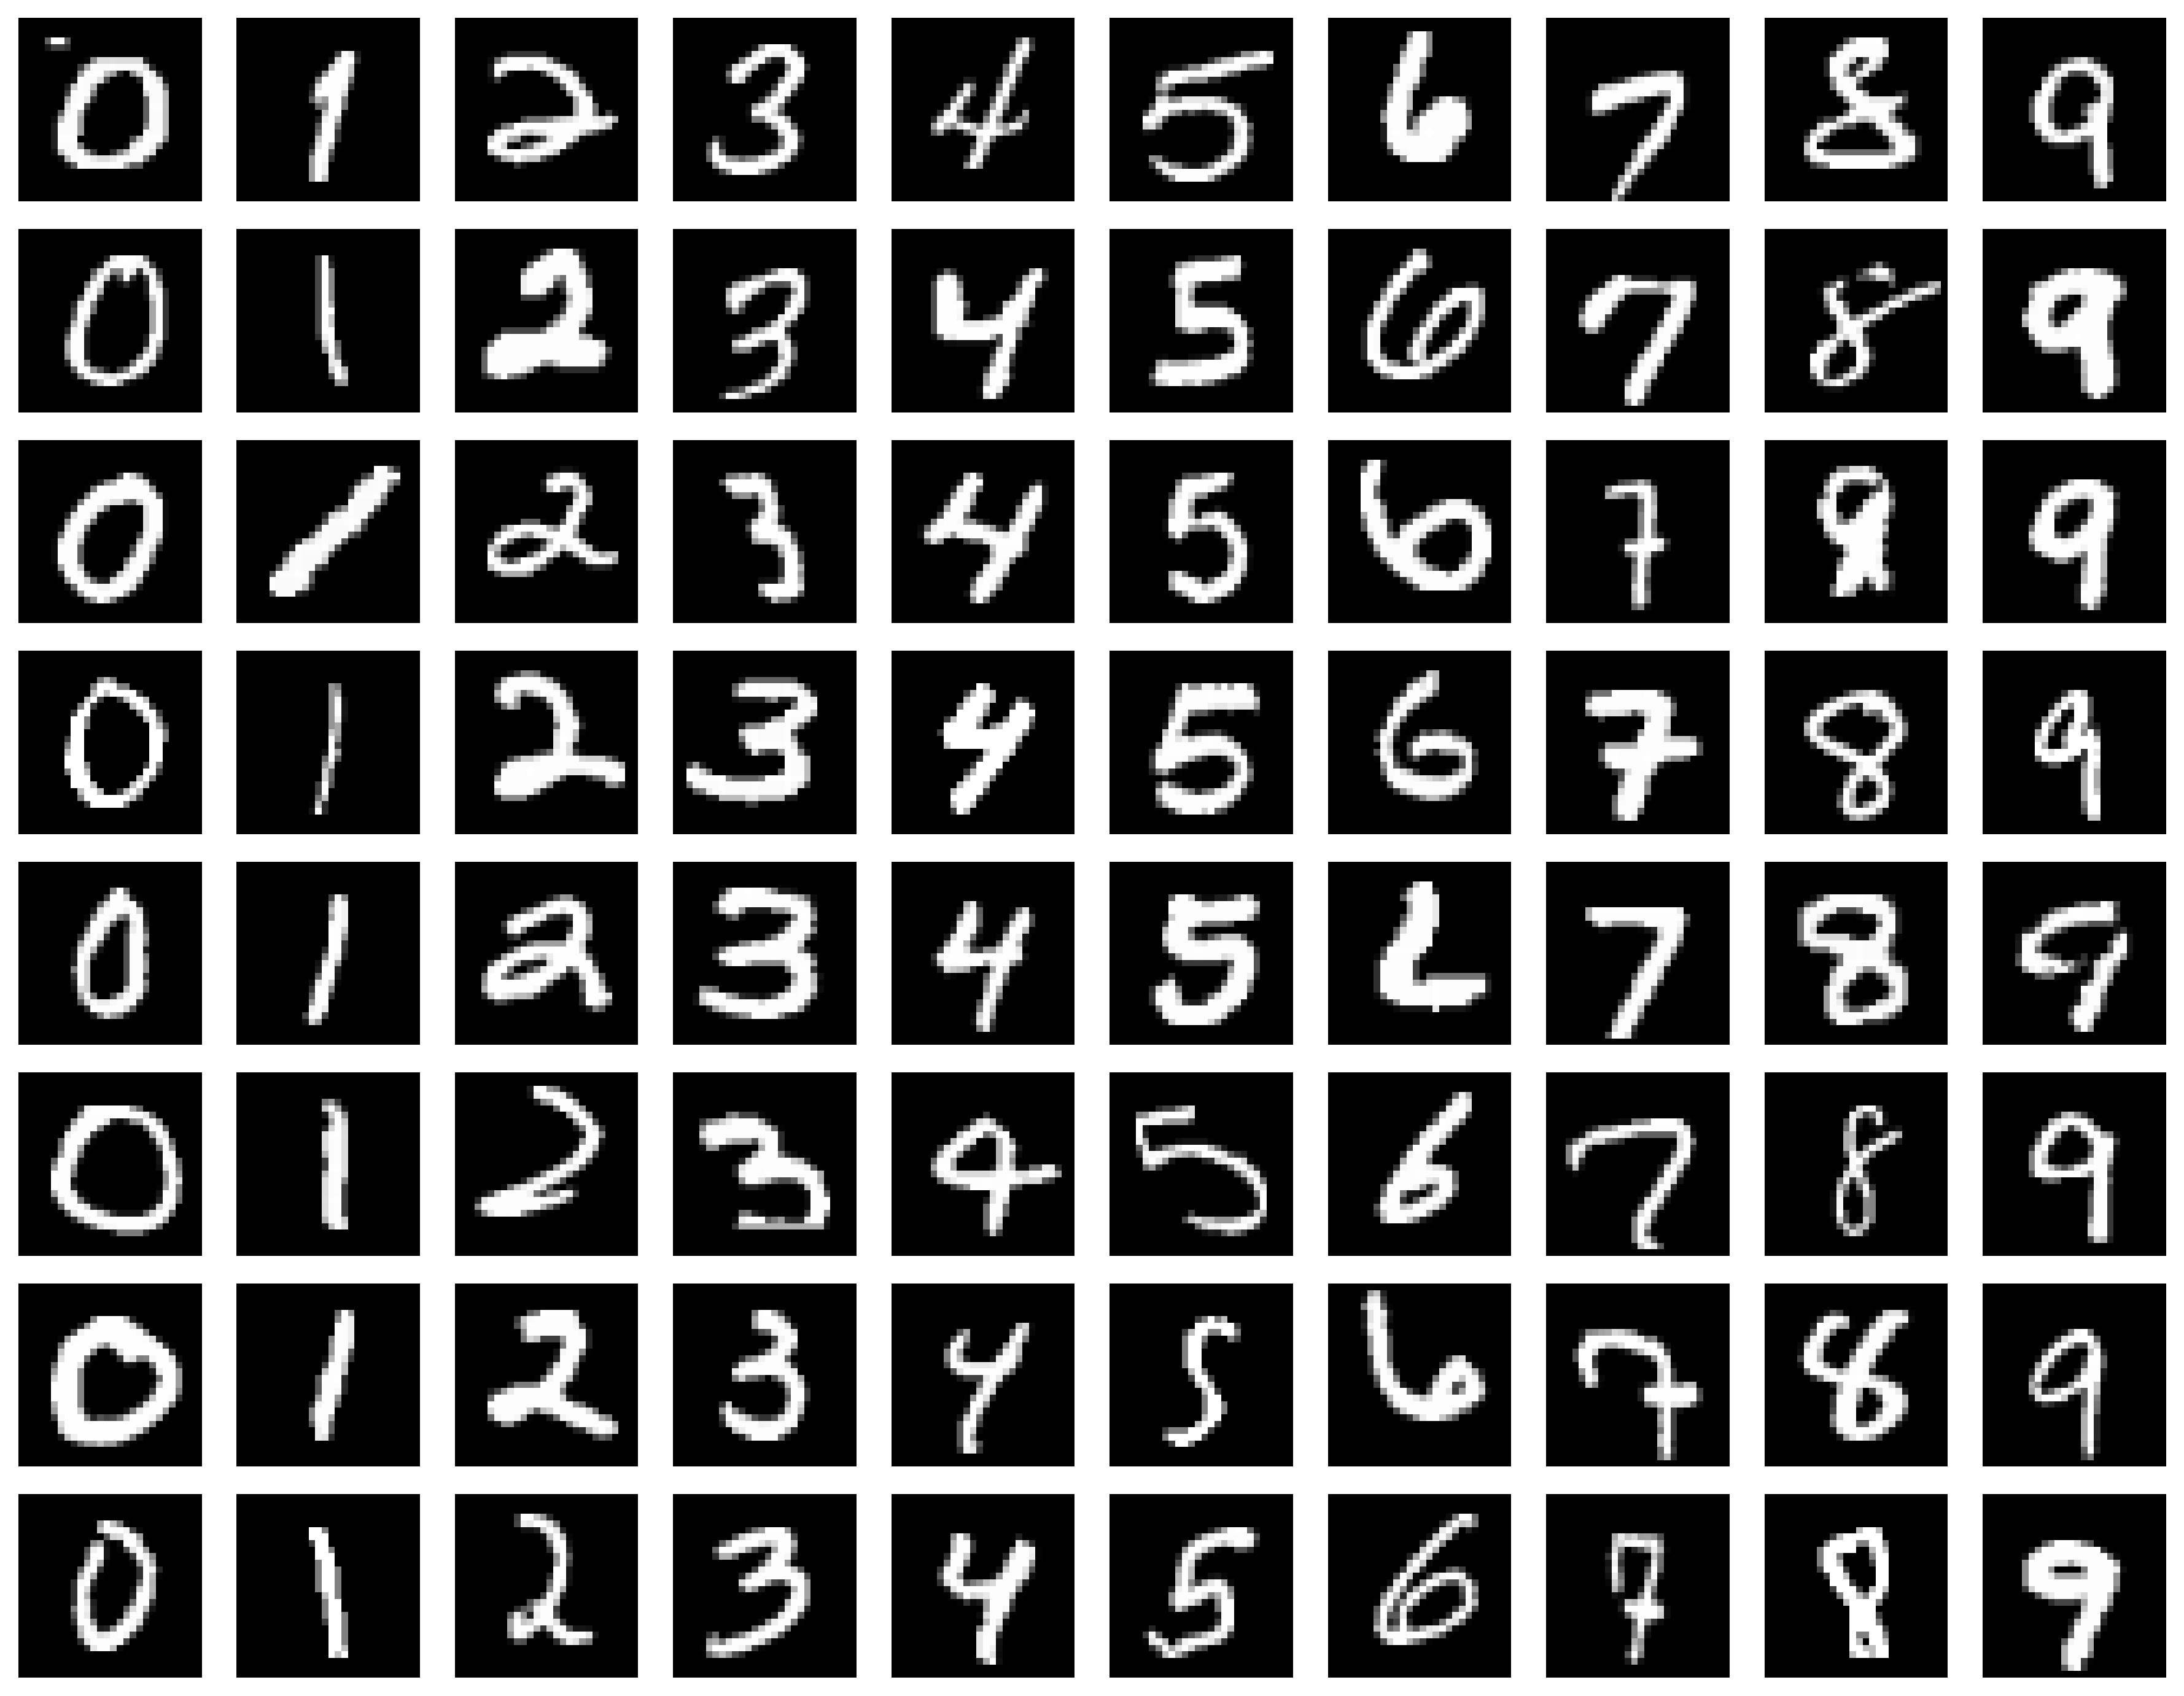
\includegraphics[width=0.8\textwidth]{../docs/assets/shared/mnist_samples}
    \caption{Một số ảnh mẫu từ tập dữ liệu MNIST.}
    \label{fig:samples}
\end{figure}

\subsection{Tiền xử lý và tăng cường dữ liệu}
\label{sec:preprocess}

Trước khi đưa vào mô hình, mỗi ảnh được chuyển thành tensor với giá trị điểm ảnh nằm trong khoảng $[0,1]$, sau đó được chuẩn hóa dựa trên giá trị trung bình và độ lệch chuẩn được tính trên tập con huấn luyện:
\begin{equation}
    \tilde{x} = \frac{x - 0{,}1308}{0{,}3082}
\end{equation}
Bước chuẩn hóa này đưa đầu vào về phân phối có trung bình gần $0$ và độ lệch chuẩn gần $1$, giúp quá trình tối ưu hóa trọng số diễn ra ổn định hơn. Đây là phương pháp tiền xử lý cơ bản được áp dụng xuyên suốt cho tất cả các mô hình.

Trong các thí nghiệm có sử dụng tăng cường dữ liệu, chúng tôi bổ sung phép biến đổi \texttt{RandomAffine(10, translate=(0.1, 0.1))} vào dữ liệu huấn luyện. Phép biến đổi này xoay ảnh một góc ngẫu nhiên trong khoảng $[-10^\circ, 10^\circ]$ và tịnh tiến ngẫu nhiên tối đa $10\%$ kích thước ảnh theo mỗi chiều, tương đương khoảng $2{,}8$ điểm ảnh. Phép biến đổi được áp dụng theo hình thức trực tuyến: mỗi khi một ảnh được nạp từ tập huấn luyện, các tham số xoay và dịch chuyển được sinh ngẫu nhiên lại, điều này giúp mô hình tiếp cận các biến thể khác nhau của cùng một mẫu ở mỗi epoch. Bảng~\ref{tab:pipeline} tóm tắt quy trình tiền xử lý, trong khi Hình~\ref{fig:aug-examples} minh họa kết quả thực tế của phép tăng cường.

Kỹ thuật tăng cường dữ liệu chỉ được thực hiện trên các batch dùng để cập nhật trọng số trong quá trình huấn luyện. Khi tiến hành đánh giá, toàn bộ dữ liệu ở cả ba tập huấn luyện, kiểm định và kiểm thử đều được đưa vào mô hình dưới dạng ảnh gốc. Nhờ vậy, mọi chỉ số đánh giá trong báo cáo đều được đo lường trên dữ liệu sạch, đảm bảo tính khách quan khi so sánh giữa các thiết lập thí nghiệm.

\begin{figure}[t]
    \centering
    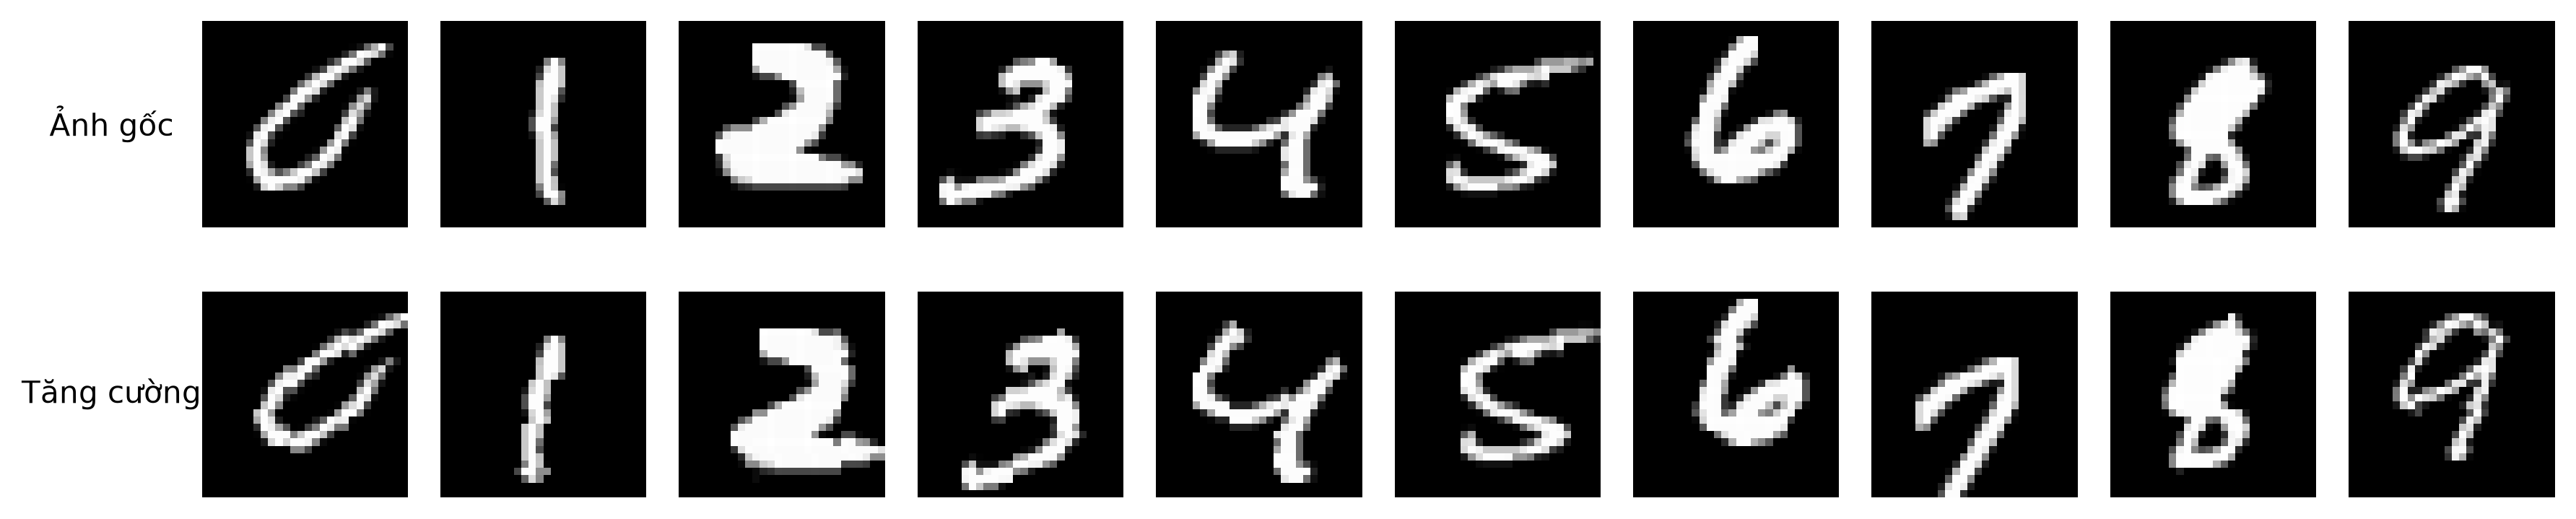
\includegraphics[width=0.9\textwidth]{../docs/assets/shared/mnist_augmentation}
    \caption{Ảnh gốc và các phiên bản sau khi áp dụng \texttt{RandomAffine(10, translate=(0.1, 0.1))}.}
    \label{fig:aug-examples}
\end{figure}

\begin{table}[t]
    \centering
    \caption{Quy trình tiền xử lý áp dụng cho dữ liệu huấn luyện.}
    \label{tab:pipeline}
    \small
    \begin{tabular}{llcc}
        \toprule
        Bước & Phép biến đổi                                   & Không tăng cường & Có tăng cường \\
        \midrule
        1    & \texttt{RandomAffine(10, translate=(0.1, 0.1))} & không            & có            \\
        2    & \texttt{ToTensor()}                             & có               & có            \\
        3    & \texttt{Normalize(0.1308, 0.3082)}              & có               & có            \\
        \bottomrule
    \end{tabular}
\end{table}

\subsection{Phương pháp đánh giá}
\label{sec:eval}

\paragraph{Quy trình đánh giá} Ba tập dữ liệu đóng các vai trò độc lập trong quá trình thực nghiệm:
\begin{itemize}
    \item \textbf{Tập huấn luyện} được sử dụng trực tiếp để cập nhật trọng số của mô hình.
    \item \textbf{Tập kiểm định} hỗ trợ theo dõi tiến trình huấn luyện, điều chỉnh tốc độ học, quyết định thời điểm dừng sớm và lựa chọn checkpoint tốt nhất.
    \item \textbf{Tập kiểm thử} chỉ được sử dụng một lần duy nhất ở giai đoạn cuối trên checkpoint đã được chọn qua tập kiểm định, đảm bảo kết quả đánh giá cuối cùng không bị ảnh hưởng bởi quá trình tinh chỉnh mô hình.
\end{itemize}
Chi tiết về điều chỉnh tốc độ học, điều kiện dừng và tiêu chí chọn checkpoint cho từng bài tập cụ thể sẽ được trình bày ở phần thiết lập huấn luyện tương ứng.

\paragraph{Độ đo hiệu suất} Gọi $K=10$ là tổng số lớp và $C_{ij}$ là số lượng mẫu thuộc lớp thật $i$ nhưng được mô hình dự đoán thành lớp $j$. Độ đo chính của báo cáo là accuracy, phản ánh tỷ lệ mẫu được phân loại đúng:
\begin{equation}
    \mathrm{accuracy} = \frac{\sum_{c=1}^{K} C_{cc}}{\sum_{i=1}^{K}\sum_{j=1}^{K} C_{ij}}.
\end{equation}
Bên cạnh đó, chúng tôi phân tích tổng số ảnh bị phân loại sai, ma trận nhầm lẫn và các mẫu lỗi cụ thể để giải thích sự khác biệt giữa các mô hình.

\paragraph{Nguyên tắc so sánh công bằng} Để đảm bảo tính khách quan, các yếu tố ngoài kiến trúc mô hình đều được cố định:
\begin{itemize}
    \item Tất cả mô hình sử dụng chung một tập dữ liệu đã chia ở Mục~\ref{sec:split} và chuỗi tiền xử lý ở Mục~\ref{sec:preprocess}.
    \item Trong cùng một bài tập, các mô hình sử dụng cùng một thuật toán tối ưu hóa, tốc độ học ban đầu, bộ lập lịch, tiêu chí dừng và seed khởi tạo. Các biến thể không tăng cường và có tăng cường chỉ khác biệt duy nhất ở bước áp dụng \texttt{RandomAffine}.
    \item Việc tinh chỉnh siêu tham số chỉ dựa trên tập kiểm định, tuyệt đối không dùng tập kiểm thử để lựa chọn mô hình.
\end{itemize}
Dù thiết lập huấn luyện có thể khác biệt giữa ba bài E1, E2 và E3 nhằm phù hợp với đặc thù của từng họ kiến trúc, nhưng các điều kiện vẫn được đảm bảo luôn giữ đồng nhất trong phạm vi từng bài.

\subsection{Khả năng tái lập}
\label{sec:repro}

Để đảm bảo khả năng tái lập kết quả, toàn bộ thông số của mỗi thí nghiệm, gồm dữ liệu, kiến trúc mô hình, thuật toán tối ưu hóa và hàm mất mát, được khai báo trong một tệp cấu hình YAML riêng. Vòng lặp huấn luyện do chúng tôi tự viết, gồm lần lượt các bước forward, tính loss, backward và cập nhật tham số, mà không dùng thư viện huấn luyện có sẵn. Mã nguồn, các tệp cấu hình và hướng dẫn chạy lại thí nghiệm được lưu công khai trên GitHub như đã nêu ở Mục~\ref{sec:intro}.

\section{E1: Softmax, MLP và CNN}
\label{sec:e1}

\subsection{Mô hình}
\label{sec:e1-models}

Phần này so sánh ba kiến trúc có mức ràng buộc về cấu trúc không gian tăng dần. Softmax là bộ phân loại tuyến tính. MLP bổ sung tính phi tuyến nhờ các tầng ẩn, nhưng vẫn coi ảnh là một vector phẳng $x\in\mathbb{R}^{784}$ nên không biết sự liên kết cục bộ của các điểm ảnh. CNN nhận trực tiếp ảnh $1\times28\times28$ và khai thác tính cục bộ cùng việc chia sẻ trọng số. Mỗi mô hình được huấn luyện ở hai thiết lập là không tăng cường dữ liệu (base) và có tăng cường dữ liệu (aug). Hai thiết lập dùng cùng kiến trúc và cùng số tham số, chỉ khác nhau ở dữ liệu dùng để cập nhật trọng số. Hình~\ref{fig:e1-arch} minh họa luồng kích thước tensor qua từng mô hình, còn Bảng~\ref{tab:e1-arch} cho số tham số của từng tầng.

\paragraph{Softmax} Mô hình tính logits qua ánh xạ tuyến tính $z = Wx + b$ với $W\in\mathbb{R}^{10\times784}$, tối ưu hóa bằng hàm mất mát cross-entropy. Với $7\,850$ tham số, mô hình học một mẫu tuyến tính cho mỗi lớp.

\paragraph{MLP} Mạng sử dụng hai tầng ẩn với cấu trúc $784\to256\to128\to10$ kết hợp hàm kích hoạt ReLU. Nhờ tính phi tuyến, mô hình tạo ra ranh giới quyết định phức tạp hơn, dù vẫn xử lý dữ liệu đầu vào dạng phẳng. Tổng số tham số là $235\,146$.

\paragraph{CNN} Kiến trúc gồm hai khối tích chập $3\times3$ sử dụng same padding, ReLU và max pooling $2\times2$, giúp thu nhỏ bản đồ không gian từ $28\times28$ xuống $7\times7$ và nâng số kênh lên $32$. Sau khi làm phẳng thành vector $1568$ chiều, dữ liệu đi qua các tầng Linear $1568\to128\to10$. Mô hình có tổng số tham số là $206\,922$. Điểm đáng chú ý là phần lớn trọng số nằm ở các tầng Linear của bộ phân loại, trong khi các tầng tích chập chỉ chiếm khoảng $2{,}3\%$ tổng số tham số.

\begin{figure}[t]
    \centering
    \resizebox{\linewidth}{!}{%
        \begin{tikzpicture}[node distance=0.3cm]

            % ---------- Softmax ----------
            \node[rowlbl] (sl) at (0,0) {Softmax\\[2pt]\normalfont\scriptsize $7\,850$ tham số};
            \node[inp, right=0.3cm of sl, label={[font=\tiny, text=black!70]below:$1{\times}28{\times}28$}] (s1) {Ảnh};
            \node[flt, right=of s1, label={[font=\tiny, text=black!70]below:$784$}] (s2) {Flatten};
            \node[lin, right=of s2, label={[font=\tiny, text=black!70]below:$10$ (logits)}] (s3) {Linear\\$784\to10$};
            \draw[arr] (s1)--(s2); \draw[arr] (s2)--(s3);

            % ---------- MLP ----------
            \node[rowlbl] (ml) at (0,-2.4) {MLP\\[2pt]\normalfont\scriptsize $235\,146$ tham số};
            \node[inp, right=0.3cm of ml, label={[font=\tiny, text=black!70]below:$1{\times}28{\times}28$}] (m1) {Ảnh};
            \node[flt, right=of m1, label={[font=\tiny, text=black!70]below:$784$}] (m2) {Flatten};
            \node[lin, right=of m2, label={[font=\tiny, text=black!70]below:$256$}] (m3) {Linear\\$784\to256$\\ReLU};
            \node[lin, right=of m3, label={[font=\tiny, text=black!70]below:$128$}] (m4) {Linear\\$256\to128$\\ReLU};
            \node[lin, right=of m4, label={[font=\tiny, text=black!70]below:$10$ (logits)}] (m5) {Linear\\$128\to10$};
            \draw[arr] (m1)--(m2); \draw[arr] (m2)--(m3); \draw[arr] (m3)--(m4); \draw[arr] (m4)--(m5);

            % ---------- CNN ----------
            \node[rowlbl] (cl) at (0,-4.8) {CNN\\[2pt]\normalfont\scriptsize $206\,922$ tham số};
            \node[inp, right=0.3cm of cl, label={[font=\tiny, text=black!70]below:$1{\times}28{\times}28$}] (c1) {Ảnh};
            \node[cnv, right=of c1, label={[font=\tiny, text=black!70]below:$16{\times}28{\times}28$}] (c2) {Conv $3{\times}3$\\$1\to16$\\ReLU};
            \node[pol, right=of c2, label={[font=\tiny, text=black!70]below:$16{\times}14{\times}14$}] (c3) {MaxPool\\$2{\times}2$};
            \node[cnv, right=of c3, label={[font=\tiny, text=black!70]below:$32{\times}14{\times}14$}] (c4) {Conv $3{\times}3$\\$16\to32$\\ReLU};
            \node[pol, right=of c4, label={[font=\tiny, text=black!70]below:$32{\times}7{\times}7$}] (c5) {MaxPool\\$2{\times}2$};
            \node[flt, right=of c5, label={[font=\tiny, text=black!70]below:$1568$}] (c6) {Flatten};
            \node[lin, right=of c6, label={[font=\tiny, text=black!70]below:$128$}] (c7) {Linear\\$1568\to128$\\ReLU};
            \node[lin, right=of c7, label={[font=\tiny, text=black!70]below:$10$ (logits)}] (c8) {Linear\\$128\to10$};
            \draw[arr] (c1)--(c2); \draw[arr] (c2)--(c3); \draw[arr] (c3)--(c4); \draw[arr] (c4)--(c5);
            \draw[arr] (c5)--(c6); \draw[arr] (c6)--(c7); \draw[arr] (c7)--(c8);

        \end{tikzpicture}}
    \caption{Sơ đồ kiến trúc ba mô hình của E1. Mỗi khối ghi phép toán, còn kích thước tensor đầu ra nằm ngay dưới khối. Màu xám: đầu vào và flatten; xanh dương: tích chập; cam: pooling; xanh lá: Linear. Đầu ra là logits $10$ chiều; hàm softmax được tính bên trong hàm mất mát.}
    \label{fig:e1-arch}
\end{figure}

\begin{table}[t]
    \centering
    \caption{Cấu trúc, kích thước đầu ra và số tham số của từng tầng trong các mô hình E1.}
    \label{tab:e1-arch}
    \small
    \begin{tabular}{llcr}
        \toprule
        Mô hình & Tầng                               & Kích thước đầu ra    & Số tham số \\
        \midrule
        Softmax & Flatten                            & $784$                & $0$        \\
                & Linear($784\to10$)                 & $10$                 & $7\,850$   \\
        \cmidrule(lr){2-4}
                & \textit{Tổng}                      &                      & $7\,850$   \\
        \midrule
        MLP     & Flatten                            & $784$                & $0$        \\
                & Linear($784\to256$) + ReLU         & $256$                & $200\,960$ \\
                & Linear($256\to128$) + ReLU         & $128$                & $32\,896$  \\
                & Linear($128\to10$)                 & $10$                 & $1\,290$   \\
        \cmidrule(lr){2-4}
                & \textit{Tổng}                      &                      & $235\,146$ \\
        \midrule
        CNN     & Conv($1\to16$, $3\times3$) + ReLU  & $16\times28\times28$ & $160$      \\
                & MaxPool($2$)                       & $16\times14\times14$ & $0$        \\
                & Conv($16\to32$, $3\times3$) + ReLU & $32\times14\times14$ & $4\,640$   \\
                & MaxPool($2$)                       & $32\times7\times7$   & $0$        \\
                & Flatten                            & $1568$               & $0$        \\
                & Linear($1568\to128$) + ReLU        & $128$                & $200\,832$ \\
                & Linear($128\to10$)                 & $10$                 & $1\,290$   \\
        \cmidrule(lr){2-4}
                & \textit{Tổng}                      &                      & $206\,922$ \\
        \bottomrule
    \end{tabular}
\end{table}

\subsection{Thiết lập huấn luyện}
\label{sec:e1-setup}

Quá trình thực nghiệm bao gồm sáu thí nghiệm tương ứng với ba mô hình được huấn luyện trong hai điều kiện có và không có tăng cường dữ liệu. Toàn bộ các thí nghiệm này đều áp dụng chung một thiết lập: bộ tối ưu hóa Adam với tốc độ học $10^{-3}$, kích thước batch bằng $64$, hàm mất mát cross-entropy và số epoch tối đa là $1000$. Tốc độ học được tự động giảm đi $10$ lần khi loss trên tập kiểm định không cải thiện sau $10$ epoch, đồng thời huấn luyện sẽ dừng sớm nếu loss trên tập kiểm định chững lại sau $20$ epoch. Checkpoint tốt nhất được lựa chọn dựa trên \textbf{loss kiểm định nhỏ nhất}.

\subsection{Kết quả và phân tích}
\label{sec:e1-results}

\paragraph{Accuracy và số tham số} Bảng~\ref{tab:e1-results} tổng hợp kết quả của sáu thí nghiệm. Với phiên bản base, accuracy kiểm thử của Softmax, MLP và CNN lần lượt là $92{,}58\%$, $97{,}68\%$ và $98{,}85\%$. Tăng cường dữ liệu nâng accuracy của MLP lên $99{,}07\%$ và của CNN lên $99{,}50\%$, nhưng làm accuracy của Softmax giảm xuống $85{,}12\%$.

\begin{table}[htbp]
    \centering
    \caption{Kết quả thực nghiệm E1 trên MNIST. Accuracy tính bằng \%, đo trên ảnh gốc; Gap là hiệu số giữa accuracy huấn luyện và kiểm định.}
    \label{tab:e1-results}
    \small
    \begin{tabular}{llrrrrrr}
        \toprule
        Mô hình & Biến thể & Tham số    & Epoch tốt nhất & Train & Val   & Test  & Gap       \\
        \midrule
        Softmax & base     & $7\,850$   & 45             & 94,00 & 92,28 & 92,58 & $1{,}72$  \\
        Softmax & aug      & $7\,850$   & 33             & 83,81 & 83,82 & 85,12 & $-0{,}01$ \\
        MLP     & base     & $235\,146$ & 6              & 99,26 & 97,58 & 97,68 & $1{,}68$  \\
        MLP     & aug      & $235\,146$ & 102            & 99,69 & 98,99 & 99,07 & $0{,}70$  \\
        CNN     & base     & $206\,922$ & 7              & 99,68 & 98,73 & 98,85 & $0{,}95$  \\
        CNN     & aug      & $206\,922$ & 72             & 99,93 & 99,41 & 99,50 & $0{,}52$  \\
        \bottomrule
    \end{tabular}
\end{table}

\paragraph{Đường cong huấn luyện} Hình~\ref{fig:e1-curves} cho thấy diễn biến loss và accuracy của sáu thí nghiệm. Ở phiên bản base, MLP và CNN đạt accuracy cao hơn Softmax và dừng huấn luyện sớm hơn, với checkpoint tốt nhất lần lượt ở epoch $6$ và $7$. Ở phiên bản aug, quá trình cải thiện của hai mô hình này kéo dài hơn, với checkpoint tốt nhất ở epoch $102$ và $72$, đồng thời khoảng cách giữa loss và accuracy của tập huấn luyện so với tập kiểm định thu hẹp lại. Ngược lại, loss của Softmax aug dao động liên tục theo dạng zigzag và quá trình huấn luyện dừng sớm vì mô hình không còn cải thiện được loss kiểm định.

\begin{figure}[htbp]
    \centering
    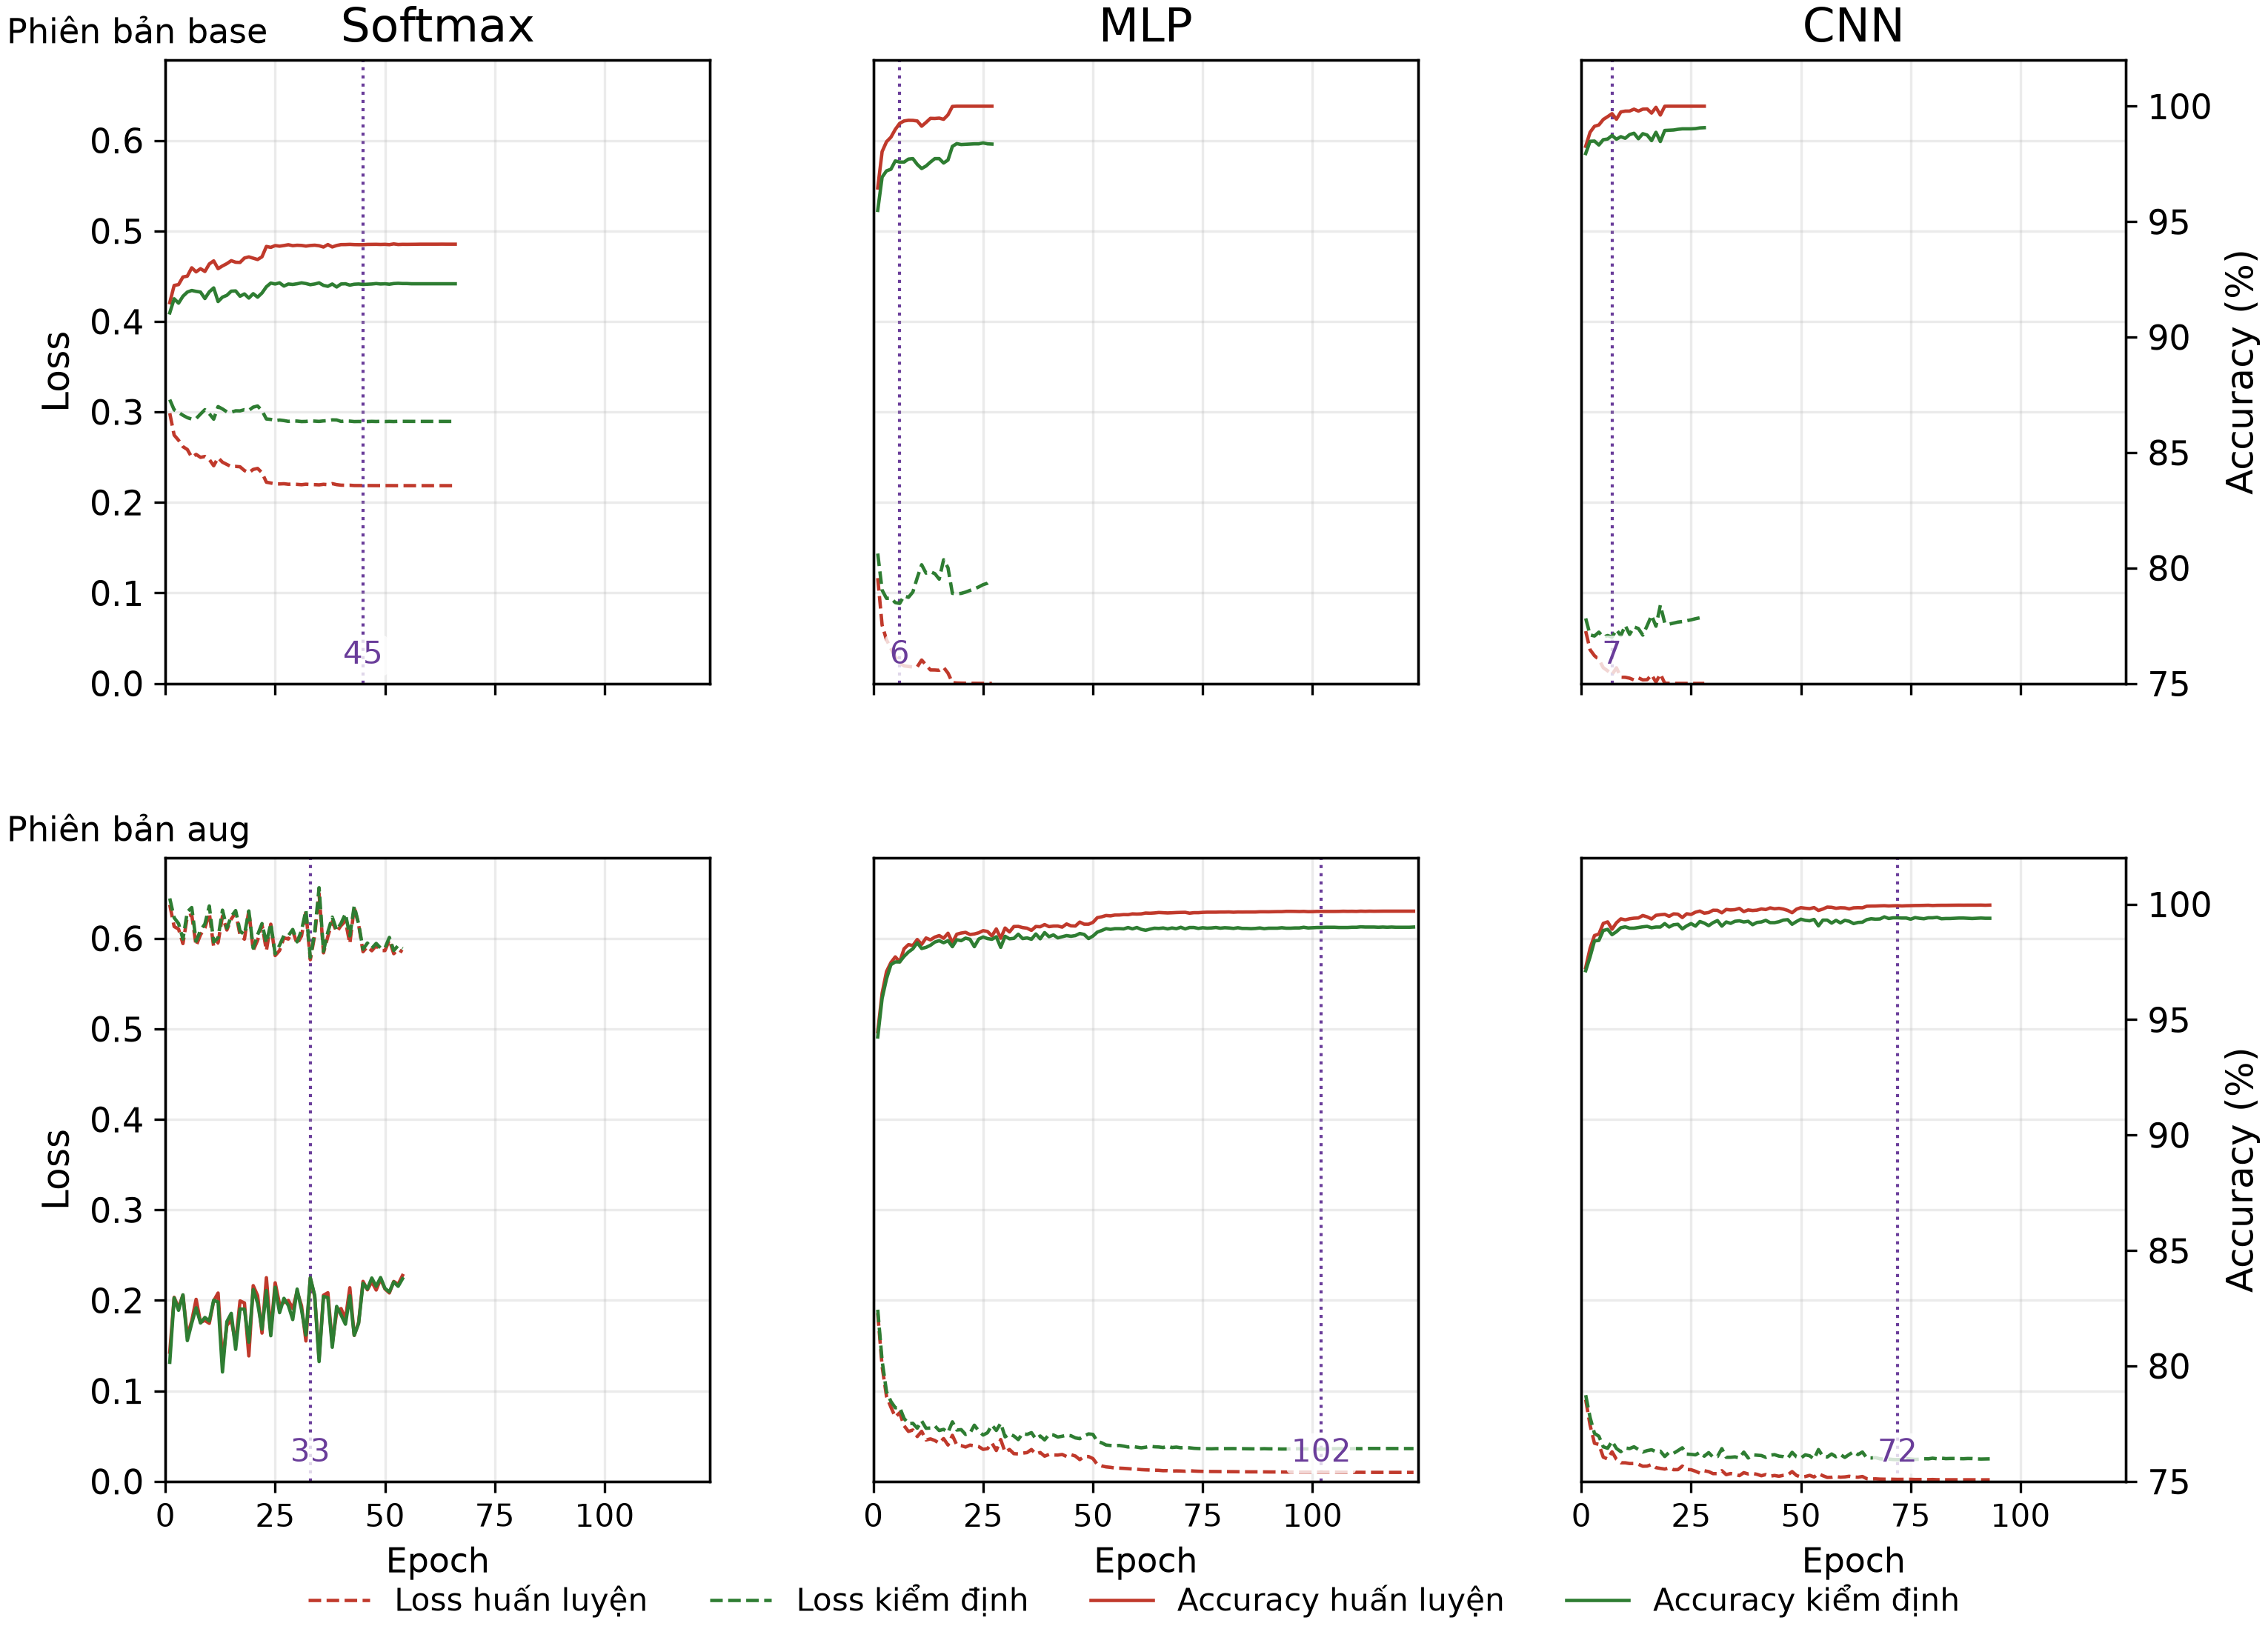
\includegraphics[width=\textwidth]{../docs/assets/e1/curves_e1.png}
    \caption{Đường cong loss và accuracy của sáu thí nghiệm trong E1. Trục trái hiển thị loss (nét đứt), trục phải hiển thị accuracy (nét liền); màu đỏ ứng với tập huấn luyện, màu xanh ứng với kiểm định. Vạch kẻ dọc màu tím đánh dấu epoch đạt hiệu suất tối ưu theo loss kiểm định.}
    \label{fig:e1-curves}
\end{figure}

\paragraph{Tổng số lỗi} Bảng~\ref{tab:e1-errors} thống kê số ảnh kiểm thử bị phân loại sai. Tăng cường dữ liệu giảm số lỗi của MLP từ $232$ xuống $93$ và của CNN từ $115$ xuống $50$, nhưng làm số lỗi của Softmax tăng gấp đôi.

\begin{table}[htbp]
    \centering
    \caption{Số lượng ảnh kiểm thử bị phân loại sai trên tổng số $10\,000$ mẫu.}
    \label{tab:e1-errors}
    \small
    \begin{tabular}{lrrr}
        \toprule
        Mô hình & Base & Aug      & Thay đổi \\
        \midrule
        Softmax & 742  & $1\,488$ & $+100\%$ \\
        MLP     & 232  & 93       & $-60\%$  \\
        CNN     & 115  & 50       & $-57\%$  \\
        \bottomrule
    \end{tabular}
\end{table}

\paragraph{Các cặp nhầm lẫn} Thang màu ở Hình~\ref{fig:e1-cm} cho thấy số lỗi giảm dần từ Softmax sang MLP rồi sang CNN. Ở phiên bản base, Softmax nhầm lẫn ở các cặp chữ số có nét giống nhau như $2/8$, $3/5$, $3/8$, $4/9$, $5/8$ và $7/9$. MLP giảm mạnh các lỗi này nhưng vẫn còn nhầm lẫn ở các cặp $4/9$ ($22$ mẫu $4\to9$) và $6/5$ ($15$ mẫu $6\to5$), còn CNN là mô hình cải thiện rõ rệt nhất. Tăng cường dữ liệu làm giảm nhầm lẫn của MLP và CNN, chẳng hạn $4\to9$ ở MLP giảm từ $22$ xuống $8$ mẫu, nhưng làm Softmax nhầm lẫn nhiều hơn, với các nhầm lẫn lớn nhất là $5\to3$ ($80$ mẫu) và $9\to4$ ($71$ mẫu).

\begin{figure}[htbp]
    \centering
    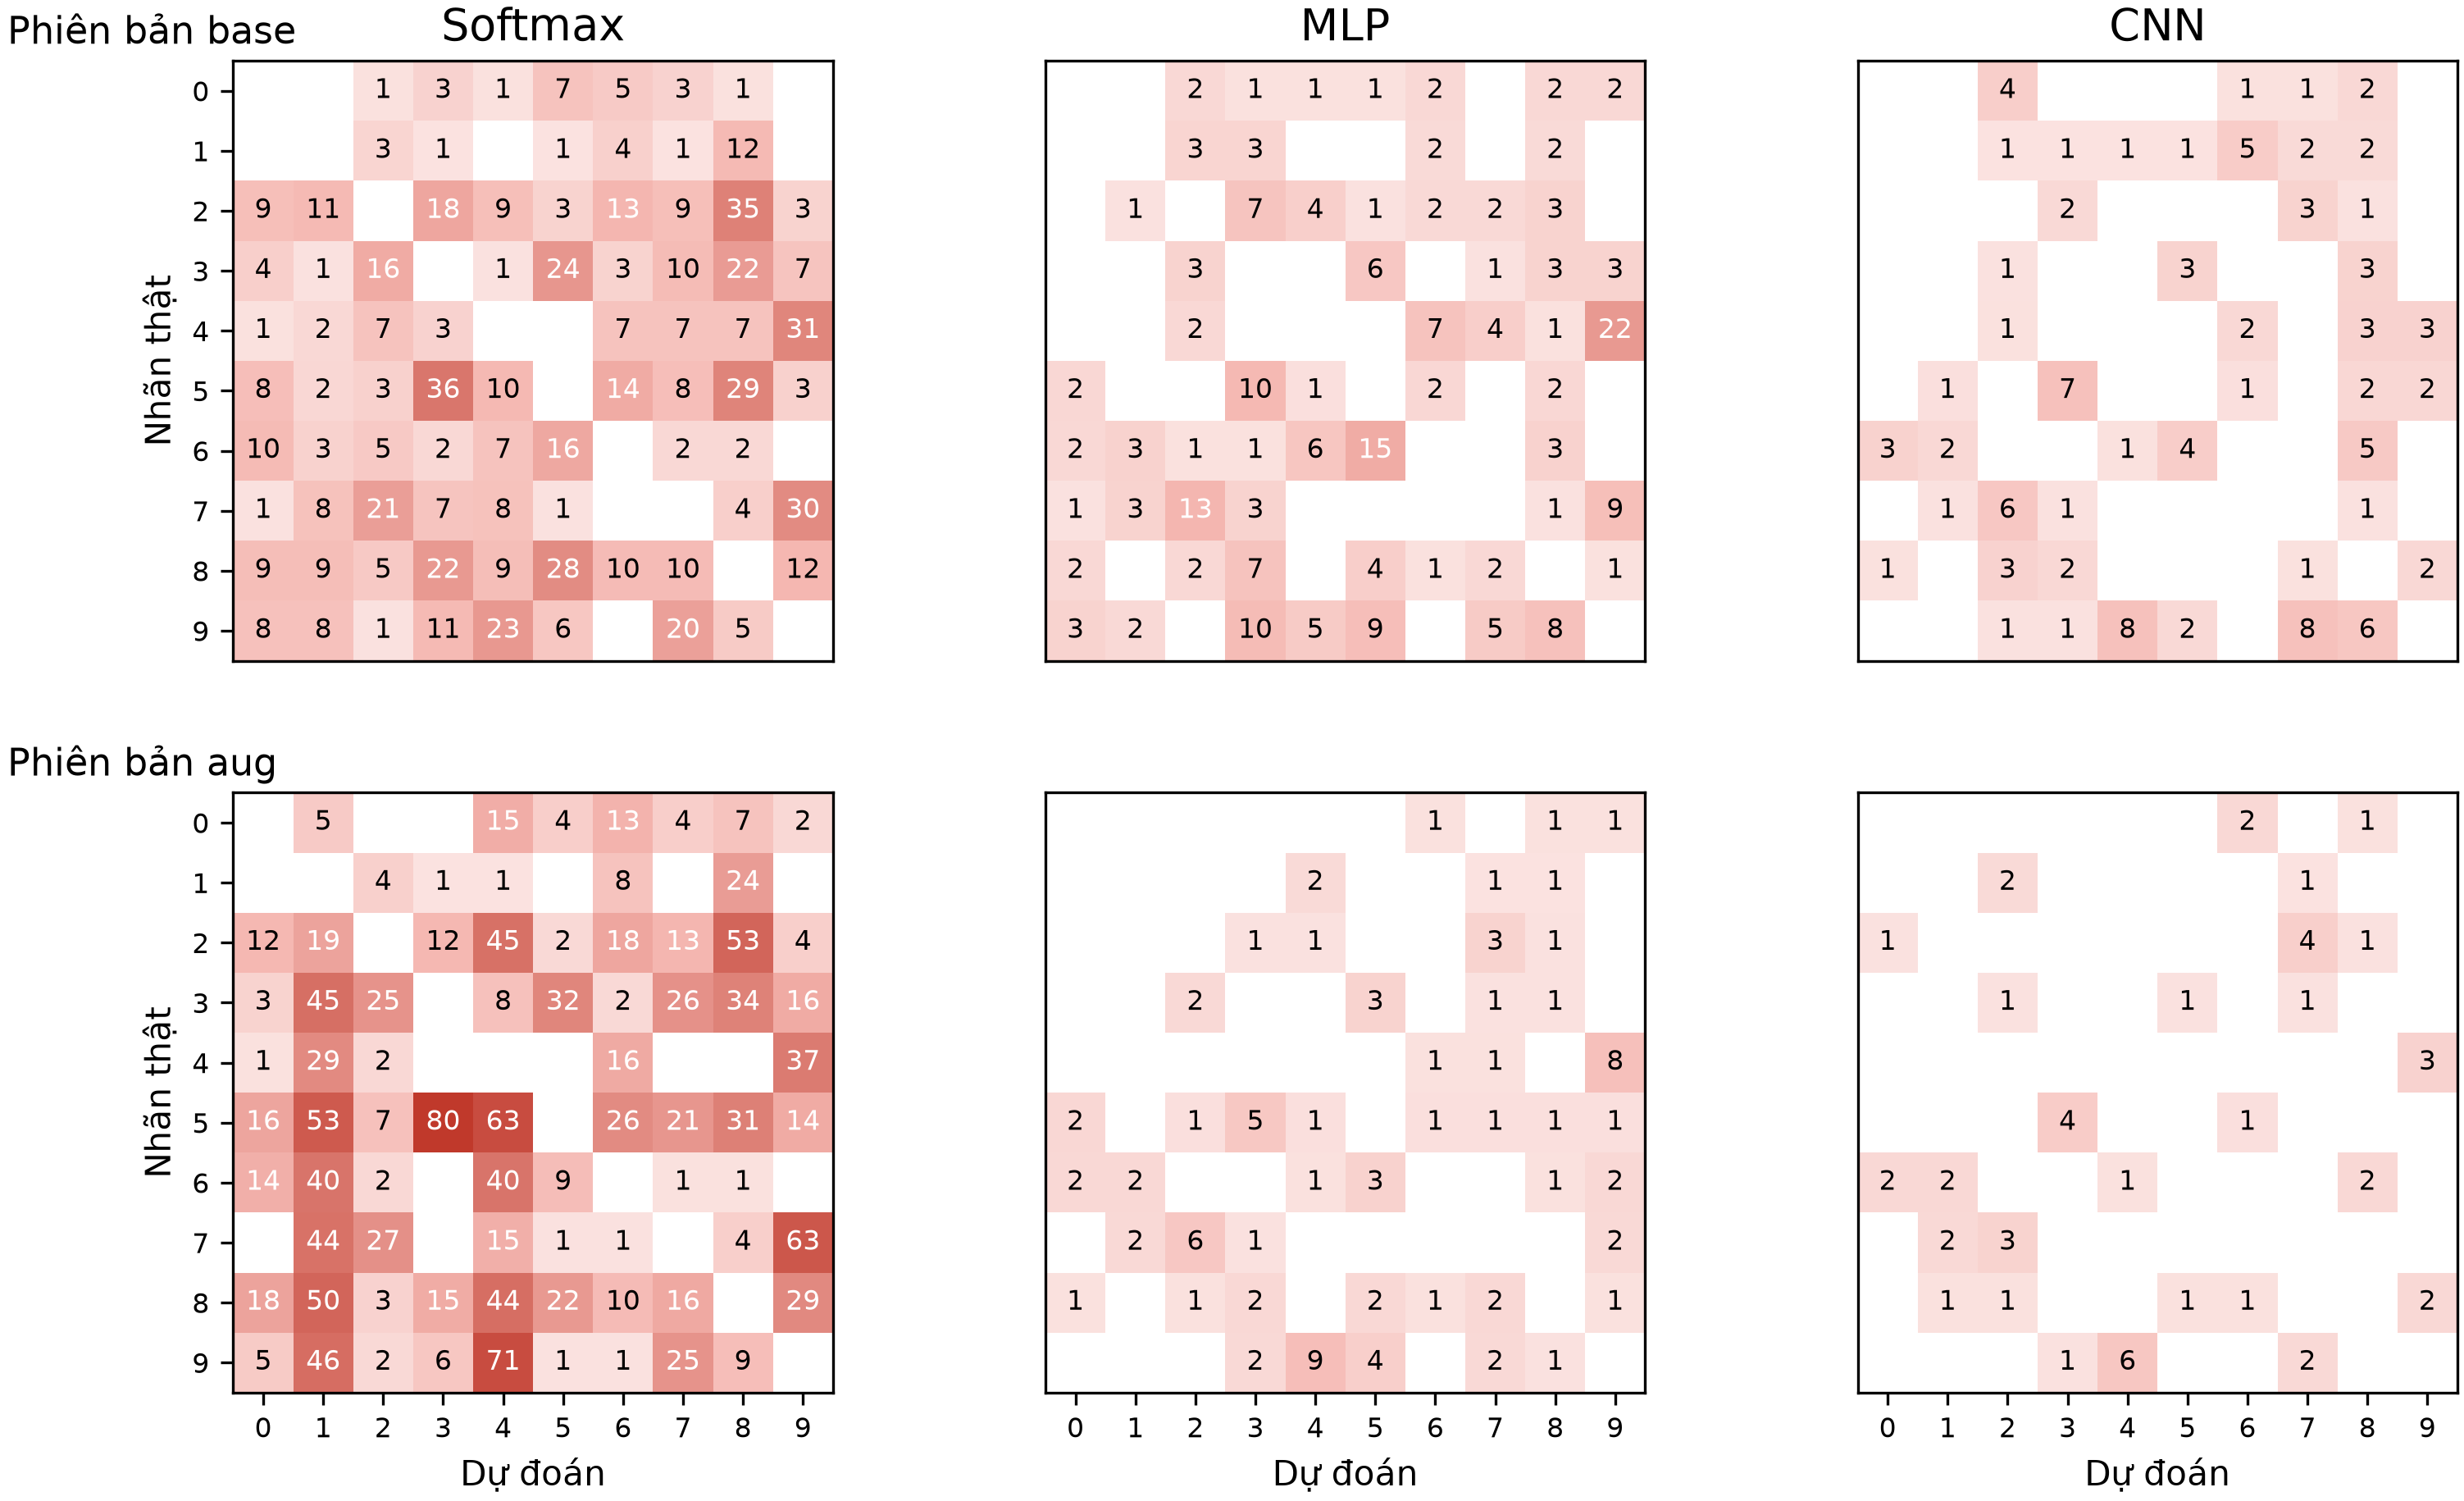
\includegraphics[width=\textwidth]{../docs/assets/e1/confusion_e1.png}
    \caption{Ma trận nhầm lẫn trên tập kiểm thử. Ô chéo được để trắng; màu đỏ đậm hơn biểu thị tỉ lệ lỗi cao hơn; số trong mỗi ô là số mẫu bị phân loại sai.}
    \label{fig:e1-cm}
\end{figure}

\paragraph{Mẫu bị phân loại sai} Hình~\ref{fig:e1-samples} minh họa các lỗi có độ tự tin cao nhất của CNN aug, là mô hình tốt nhất của bài E1. Một số mẫu khó phân biệt ngay từ hình ảnh: chữ số $6$ và chữ số $2$ bị nhận nhầm thành $0$ vì hình dạng khá giống chữ số $0$, còn chữ số $9$ viết thiếu nét nên trông giống chữ số $4$. Tuy nhiên, cũng có những lỗi cho thấy mô hình chưa tốt, chẳng hạn chữ số $1$ bị nhận nhầm thành $2$ dù hình dạng khá rõ ràng.

\begin{figure}[htbp]
    \centering
    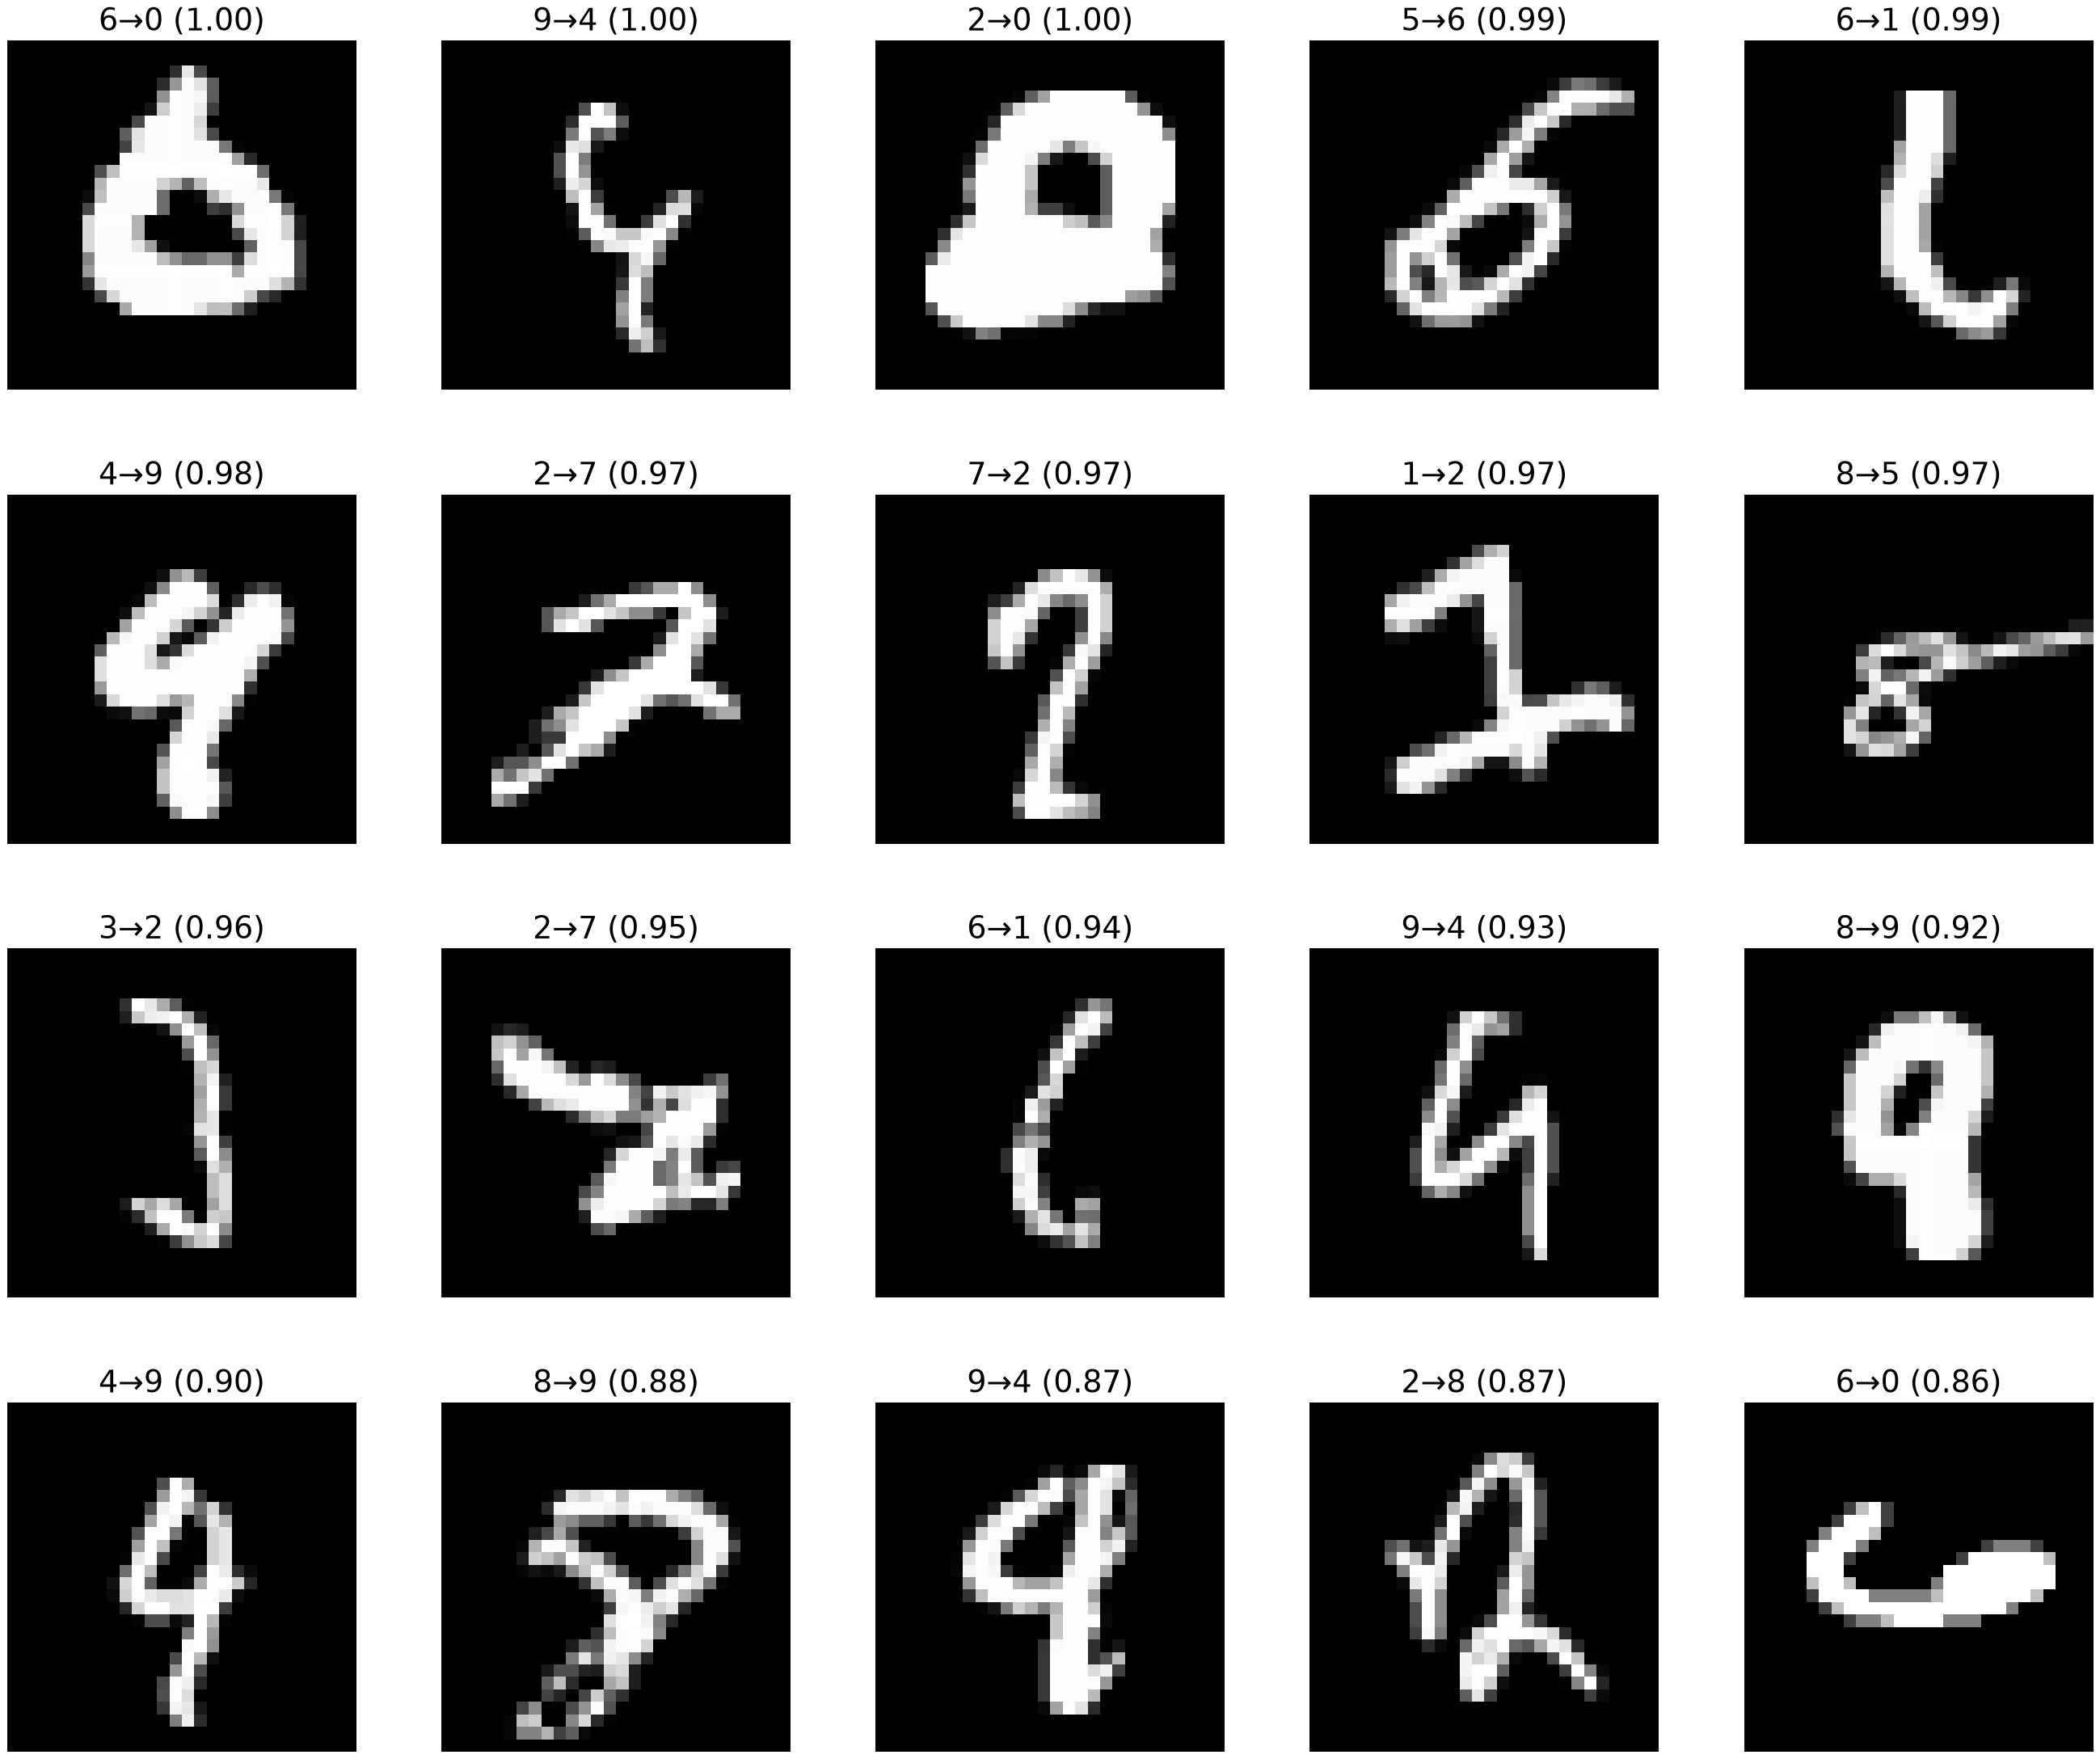
\includegraphics[width=\textwidth]{../docs/assets/e1/failures_cnn_aug.png}
    \caption{Một số mẫu kiểm thử bị phân loại sai có độ tự tin dự đoán cao nhất của CNN tăng cường. Mỗi ảnh ghi nhãn thật $\rightarrow$ dự đoán và xác suất của lớp dự đoán sai.}
    \label{fig:e1-samples}
\end{figure}

\subsection{Thảo luận}
\label{sec:e1-discussion}

\paragraph{Kiến trúc quan trọng hơn số tham số} Dù có ít tham số hơn MLP khoảng $12\%$, CNN chỉ mắc khoảng một nửa số lỗi, cụ thể là $115$ so với $232$ ở bản base và $50$ so với $93$ ở bản aug. Tầng Linear đầu tiên của hai mô hình có số tham số gần bằng nhau, lần lượt là $200\,832$ và $200\,960$, nên khác biệt chính nằm ở bộ trích xuất đặc trưng. Bộ này chỉ gồm hai tầng tích chập với khoảng $2{,}3\%$ tổng số tham số của CNN, nhưng khai thác cấu trúc cục bộ và chia sẻ trọng số. Do đó, ưu thế của CNN đến từ thiên kiến quy nạp chứ không đến từ số lượng tham số.

\paragraph{Tăng cường dữ liệu nâng cao hiệu quả cho mô hình đủ khả năng biểu diễn} Tăng cường dữ liệu giảm số lỗi kiểm thử của MLP và CNN lần lượt $60\%$ và $57\%$. Khoảng cách giữa tập huấn luyện và kiểm định thu hẹp từ $1{,}68$ xuống $0{,}70$ điểm ở MLP và từ $0{,}95$ xuống $0{,}52$ điểm ở CNN, còn epoch tốt nhất dời từ $6$ lên $102$ ở MLP và từ $7$ lên $72$ ở CNN. Như vậy tăng cường đóng vai trò điều chuẩn, làm chậm quá khớp và đổi lại thời gian huấn luyện dài hơn.

\paragraph{Hạn chế của mô hình tuyến tính với dữ liệu tăng cường} Với Softmax, accuracy kiểm thử giảm từ $92{,}58\%$ xuống $85{,}12\%$ khi có tăng cường dữ liệu. Accuracy huấn luyện, đo trên ảnh sạch, cũng giảm từ $94{,}0\%$ xuống $83{,}8\%$ và gần bằng accuracy kiểm định, nên mô hình đang thiếu khớp chứ không phải quá khớp. Softmax chấm điểm mỗi lớp bằng $w_c^\top x$ với mỗi trọng số gắn với một vị trí điểm ảnh cố định, nên không thể hấp thụ các phép dịch chuyển tới khoảng $2{,}8$ điểm ảnh. Do đó, tăng cường dữ liệu chỉ phát huy hiệu quả khi mô hình đủ khả năng biểu diễn để học được tính bất biến mà nó mang lại.

\section{E2: Transformer --- MSA và các cách tạo token}
\label{sec:e2}

\subsection{Mô hình}
\label{sec:e2-models}

Phần này mô tả bộ phân loại Transformer nông dùng chung cho mọi thí nghiệm E2. Các mô hình chỉ khác nhau ở hai điểm: cách tạo token (hàng, patch $4\times4$, patch $7\times7$, patch $8\times8$ chồng lấn, CNN-stem) và cách cài đặt MSA (tự cài đặt hoặc \texttt{nn.MultiheadAttention}). Mỗi cách tạo token đều được huấn luyện với MSA tự cài đặt, và đều có thêm bản PyTorch để đối chiếu.

\paragraph{Multi-Head Self-Attention}
Cho chuỗi token $X\in\mathbb{R}^{N\times d}$ ($N$ token, chiều $d=d_{\text{model}}$), $h$ đầu và $d_k=d/h$, đầu thứ $i$ tính
\begin{align}
    Q_i             & = XW_i^Q,\quad K_i = XW_i^K,\quad V_i = XW_i^V,                \\
    \mathrm{head}_i & = \softmax\!\left(\frac{Q_iK_i^{\top}}{\sqrt{d_k}}\right)V_i,  \\
    \mathrm{MSA}(X) & = \mathrm{Concat}(\mathrm{head}_1,\dots,\mathrm{head}_h)\,W^O,
\end{align}
với $W_i^Q,W_i^K,W_i^V\in\mathbb{R}^{d\times d_k}$ và $W^O\in\mathbb{R}^{d\times d}$. Ma trận attention có kích thước $N\times N$ cho mỗi đầu, nên chi phí thời gian tăng theo $O(N^2 d)$ và bộ nhớ theo $O(hN^2)$; điều này quan trọng khi so sánh các cách tạo token.

\paragraph{Bản tự cài đặt} Chỉ dùng \texttt{Linear}, \texttt{einsum} và \texttt{softmax}. Một lớp \texttt{Linear} duy nhất ($d\to3d$) tạo cả $Q,K,V$, với trọng số xếp chồng $[W^Q;W^K;W^V]$ cùng cách xếp với \texttt{in\_proj\_weight} của PyTorch; kết quả được reshape thành $(B,N,3,h,d_k)$ rồi hoán vị thành $(3,B,h,N,d_k)$. Điểm số $QK^\top/\sqrt{d_k}$ tính bằng \texttt{einsum('bhnd,\allowbreak bhmd-\allowbreak>\allowbreak bhnm')}, qua softmax theo chiều khóa, rồi dropout trên ma trận attention; đầu ra mỗi đầu là \texttt{einsum('bhnm,\allowbreak bhmd-\allowbreak>\allowbreak bhnd')} của attention với $V$. Các đầu được ghép lại thành $(B,N,d)$ và đi qua phép chiếu đầu ra $W^O$ (\texttt{Linear} $d\to d$). Bản này không dùng \texttt{nn.MultiheadAttention} hay \texttt{nn.TransformerEncoder*}.

\paragraph{Bản PyTorch} Cùng bộ phân loại nhưng thay MSA bằng \texttt{nn.MultiheadAttention} (\texttt{batch\_first=True}, cùng số đầu và dropout) để đối chiếu. Hai bản dùng chung tokenizer, LayerNorm, FFN, token CLS và đầu phân loại, và với cùng seed thì khởi tạo trọng số giống hệt nhau. Để kiểm tra bản tự cài đặt, chúng tôi sao chép trọng số sang module PyTorch và so sánh đầu ra, attention và gradient trên một số đầu vào ngẫu nhiên (\texttt{scripts/e2/check\_msa.py}); chênh lệch tối đa khoảng $10^{-7}$ ở float32 với đầu ra và $2\times10^{-5}$ với gradient.

\paragraph{Kiến trúc bộ phân loại} Mỗi cách tạo token đưa ảnh về chuỗi $N$ token và chiếu lên $d_{\text{model}}=64$. Một token CLS được thêm vào đầu chuỗi, rồi cộng mã hóa vị trí học được kích thước $(N+1)\times d_{\text{model}}$. Chuỗi đi qua $L=4$ khối encoder dạng pre-LayerNorm, mỗi khối gồm MSA $h=4$ đầu ($d_k=16$) và FFN (\texttt{Linear}--GELU--\texttt{Linear}, chiều ẩn $d_{ff}=128=2d_{\text{model}}$), mỗi phần có kết nối residual. Dropout $p=0{,}1$ được đặt trên ma trận attention và trên đầu ra của MSA trước khi cộng residual; ở FFN, dropout nằm giữa GELU và \texttt{Linear} thứ hai và không có dropout trên nhánh residual của FFN. Sau một LayerNorm cuối, đầu phân loại (\texttt{Linear} $64\to10$) áp dụng lên token CLS.

\paragraph{Các cách tạo token} Chúng tôi triển khai năm cách tạo token:
\begin{itemize}
    \item \textbf{Hàng (row)}: mỗi hàng ảnh là một token, $N=28$ token chiều $28$.
    \item \textbf{Patch $4\times4$}: các ô lưới không chồng lấn, $N=(28/4)^2=49$ token chiều $16$.
    \item \textbf{Patch $7\times7$}: $N=(28/7)^2=16$ token chiều $49$.
    \item \textbf{Patch $8\times8$ chồng lấn}: patch $8\times8$ với bước (stride) $4$, nên hai patch liền kề chồng lên nhau một nửa, cho $N=((28-8)/4+1)^2=36$ token chiều $64$.
    \item \textbf{CNN-stem}: một CNN nhỏ gồm hai khối Conv$3\times3$--BatchNorm--ReLU--MaxPool$2\times2$ (32 rồi 64 kênh) và một Conv$1\times1$ lên $64$ kênh, trích bản đồ đặc trưng $C\times H'\times W'=64\times7\times7$; mỗi vị trí không gian là một token, $N=H'W'=49$, chiều $C=64$.
\end{itemize}
Cả năm cách đều dùng token CLS và mã hóa vị trí học được; chiều token trong Bảng~\ref{tab:e2-tokens} là số giá trị của mỗi token trước khi được chiếu lên $d_{\text{model}}=64$; riêng với CNN-stem, Conv$1\times1$ nằm trong tokenizer nên token ra khỏi tokenizer đã có $64$ chiều. Bảng~\ref{tab:e2-tokens} liệt kê số token.

\begin{table}[t]
    \centering
    \caption{Số token $N$ và chiều token của từng cách tạo token.}
    \label{tab:e2-tokens}
    \begin{tabular}{lrr}
        \toprule
        Cách tạo token             & $N$     & Chiều token \\
        \midrule
        Hàng                       & 28      & 28          \\
        Patch $4\times4$           & 49      & 16          \\
        Patch $7\times7$           & 16      & 49          \\
        Patch $8\times8$ chồng lấn & 36      & 64          \\
        CNN-stem                   & 49      & 64          \\
        \bottomrule
    \end{tabular}
\end{table}

\begin{figure}[htbp]
    \centering
    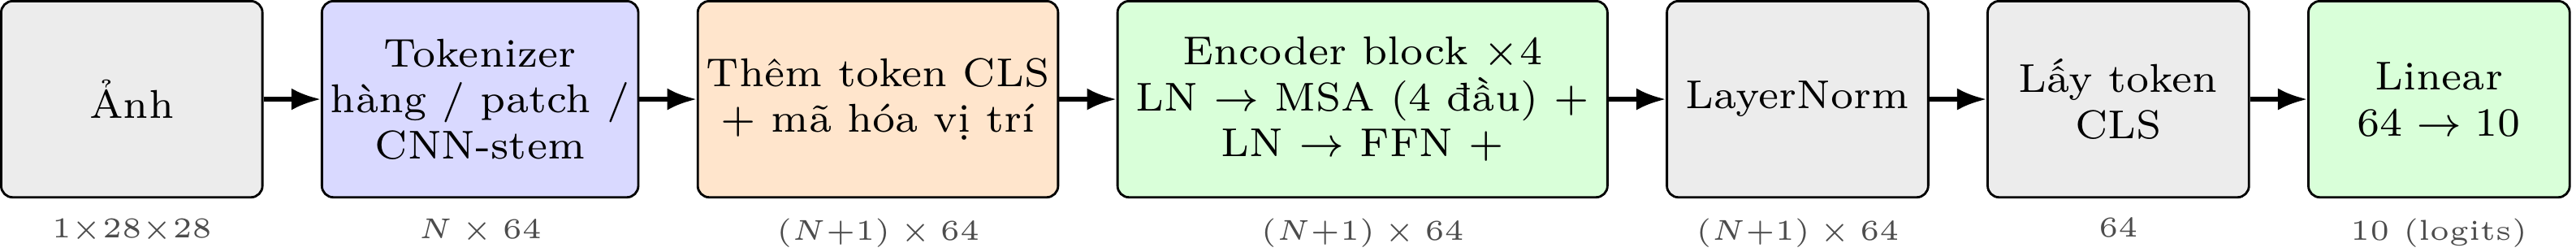
\includegraphics[width=\linewidth]{../docs/assets/e2/model_e2.png}
    \caption{Sơ đồ bộ phân loại Transformer của E2. Mỗi khối ghi phép toán, còn kích thước tensor đầu ra nằm ngay dưới khối ($N$ là số token, tùy cách tạo token). Màu xám: đầu vào, LayerNorm và lấy token CLS; xanh dương: tokenizer; cam: thêm CLS và mã hóa vị trí; xanh lá: encoder và Linear.}
    \label{fig:e2-arch}
\end{figure}

\begin{table}[htbp]
    \centering
    \caption{Số tham số của từng thành phần trong các mô hình E2 ($d_{\text{model}}=64$). Hai bản MSA có cùng số tham số.}
    \label{tab:e2-arch}
    \small
    \setlength{\tabcolsep}{3.5pt}
    \begin{tabular}{lrrrrr}
        \toprule
        Thành phần                      & Hàng       & Patch $4\times4$ & Patch $7\times7$ & Chồng lấn $8\times8$ & CNN-stem   \\
        \midrule
        Tokenizer                       & $1\,856$   & $1\,088$         & $3\,200$         & $4\,160$                   & $23\,168$  \\
        Token CLS                       & $64$       & $64$             & $64$             & $64$                       & $64$       \\
        Mã hóa vị trí $(N{+}1)\times64$ & $1\,856$   & $3\,200$         & $1\,088$         & $2\,368$                   & $3\,200$   \\
        MSA ($4$ block)                 & $66\,560$  & $66\,560$        & $66\,560$        & $66\,560$                  & $66\,560$  \\
        FFN ($4$ block)                 & $66\,304$  & $66\,304$        & $66\,304$        & $66\,304$                  & $66\,304$  \\
        LayerNorm ($4\times2$ và cuối)  & $1\,152$   & $1\,152$         & $1\,152$         & $1\,152$                   & $1\,152$   \\
        Linear $64\to10$                & $650$      & $650$            & $650$            & $650$                      & $650$      \\
        \midrule
        \textit{Tổng}                   & $138\,442$ & $139\,018$       & $139\,018$       & $141\,258$                 & $161\,098$ \\
        \bottomrule
    \end{tabular}
\end{table}

\subsection{Thiết lập huấn luyện}
\label{sec:e2-setup}

Quá trình thực nghiệm bao gồm mười thí nghiệm tương ứng với năm cách tạo token, mỗi cách được huấn luyện với MSA tự cài đặt và với MSA của PyTorch. Dữ liệu và cách chia giống E1 (50\,000 ảnh train, 10\,000 ảnh val phân tầng với seed $42$, 10\,000 ảnh test), chỉ chuẩn hóa mean/std và \emph{không} tăng cường dữ liệu. Toàn bộ các thí nghiệm đều áp dụng chung một thiết lập: bộ tối ưu hóa AdamW với tốc độ học $10^{-3}$ và weight decay $0{,}05$ (chỉ áp lên trọng số của \texttt{Linear} và \texttt{Conv2d}; bias, tham số chuẩn hóa, token CLS và mã hóa vị trí không bị decay), kích thước batch bằng $128$, hàm mất mát cross-entropy và số epoch tối đa là $200$. Tốc độ học được tự động giảm đi $10$ lần (\texttt{ReduceLROnPlateau}) khi loss trên tập val không cải thiện sau $10$ epoch, đồng thời huấn luyện sẽ dừng sớm nếu loss trên tập val chững lại sau $20$ epoch. Checkpoint tốt nhất được lựa chọn dựa trên \textbf{loss val nhỏ nhất}, nên accuracy val và test trong cùng một dòng của bảng thuộc về cùng một mô hình. Mọi thí nghiệm dùng seed $42$. So với E1, E2 dùng AdamW thay cho Adam, batch size $128$ thay cho $64$ và tối đa $200$ epoch thay cho $1000$.

\subsection{Kết quả và phân tích}
\label{sec:e2-results}

\paragraph{Accuracy và số tham số} Bảng~\ref{tab:e2-results} tổng hợp kết quả của mười thí nghiệm. Với MSA tự cài đặt, accuracy test xếp từ cao xuống thấp là CNN-stem $99{,}33\%$, hàng $99{,}13\%$, patch $8\times8$ chồng lấn $98{,}98\%$, patch $4\times4$ $98{,}85\%$ và patch $7\times7$ $98{,}70\%$. Với MSA của PyTorch, accuracy test của năm cách tạo token nằm trong khoảng $98{,}67\%$ đến $99{,}49\%$ và CNN-stem cũng dẫn đầu. Ở mọi mô hình, accuracy train gần $100\%$ và Gap giữa train và val từ $0{,}67$ đến $1{,}43$ điểm, nhỏ nhất ở CNN-stem. Hai bản MSA cho accuracy gần nhau ở cả năm cách tạo token, chênh lệch lớn nhất là $0{,}19$ điểm.

\begin{table}[htbp]
    \centering
    \caption{Kết quả thực nghiệm E2 trên MNIST. Accuracy tính bằng \%, đo trên ảnh gốc; Gap là hiệu số giữa accuracy train và val; Epoch là epoch có loss val nhỏ nhất; Giây/epoch chỉ tính các bước huấn luyện.}
    \label{tab:e2-results}
    \small
    \setlength{\tabcolsep}{3.5pt}
    \begin{tabular}{llrrrrrrr}
        \toprule
        Cách tạo token             & MSA        & Tham số  & Epoch & Train  & Val   & Test  & Gap  & Giây/epoch \\
        \midrule
        Patch $4\times4$            & Tự cài đặt & 139\,018 & 38 & 99,95 & 98,73 & 98,85 & $1{,}22$ & 11,08 \\
                                    & PyTorch    & 139\,018 & 33 & 99,96 & 98,60 & 98,67 & $1{,}36$ & 15,83 \\
        \addlinespace
        Patch $7\times7$            & Tự cài đặt & 139\,018 & 47 & 99,99 & 98,60 & 98,70 & $1{,}39$ & 11,76 \\
                                    & PyTorch    & 139\,018 & 48 & 99,98 & 98,55 & 98,80 & $1{,}43$ & 15,81 \\
        \addlinespace
        Patch $8\times8$ chồng lấn  & Tự cài đặt & 141\,258 & 52 & 99,99 & 98,94 & 98,98 & $1{,}05$ & 16,17 \\
                                    & PyTorch    & 141\,258 & 53 & 100,00 & 99,06 & 99,07 & $0{,}94$ & 15,55 \\
        \addlinespace
        Hàng                        & Tự cài đặt & 138\,442 & 43 & 99,96 & 98,87 & 99,13 & $1{,}09$ & 16,03 \\
                                    & PyTorch    & 138\,442 & 34 & 99,89 & 98,82 & 98,94 & $1{,}07$ & 10,69 \\
        \addlinespace
        CNN-stem                    & Tự cài đặt & 161\,098 & 33 & 99,99 & 99,32 & 99,33 & $0{,}67$ & 16,73 \\
                                    & PyTorch    & 161\,098 & 34 & 99,99 & 99,29 & 99,49 & $0{,}70$ & 15,94 \\
        \bottomrule
    \end{tabular}
\end{table}

\paragraph{Đường cong huấn luyện} Hình~\ref{fig:e2-curves} cho thấy hai bản MSA có đường cong bám sát nhau ở cả năm cách tạo token. Epoch tốt nhất nằm trong khoảng $33$ đến $53$; sau epoch đó loss val gần như phẳng trong khi accuracy train đã gần $100\%$, và huấn luyện dừng sớm sau $20$ epoch không cải thiện.

\begin{figure}[htbp]
    \centering
    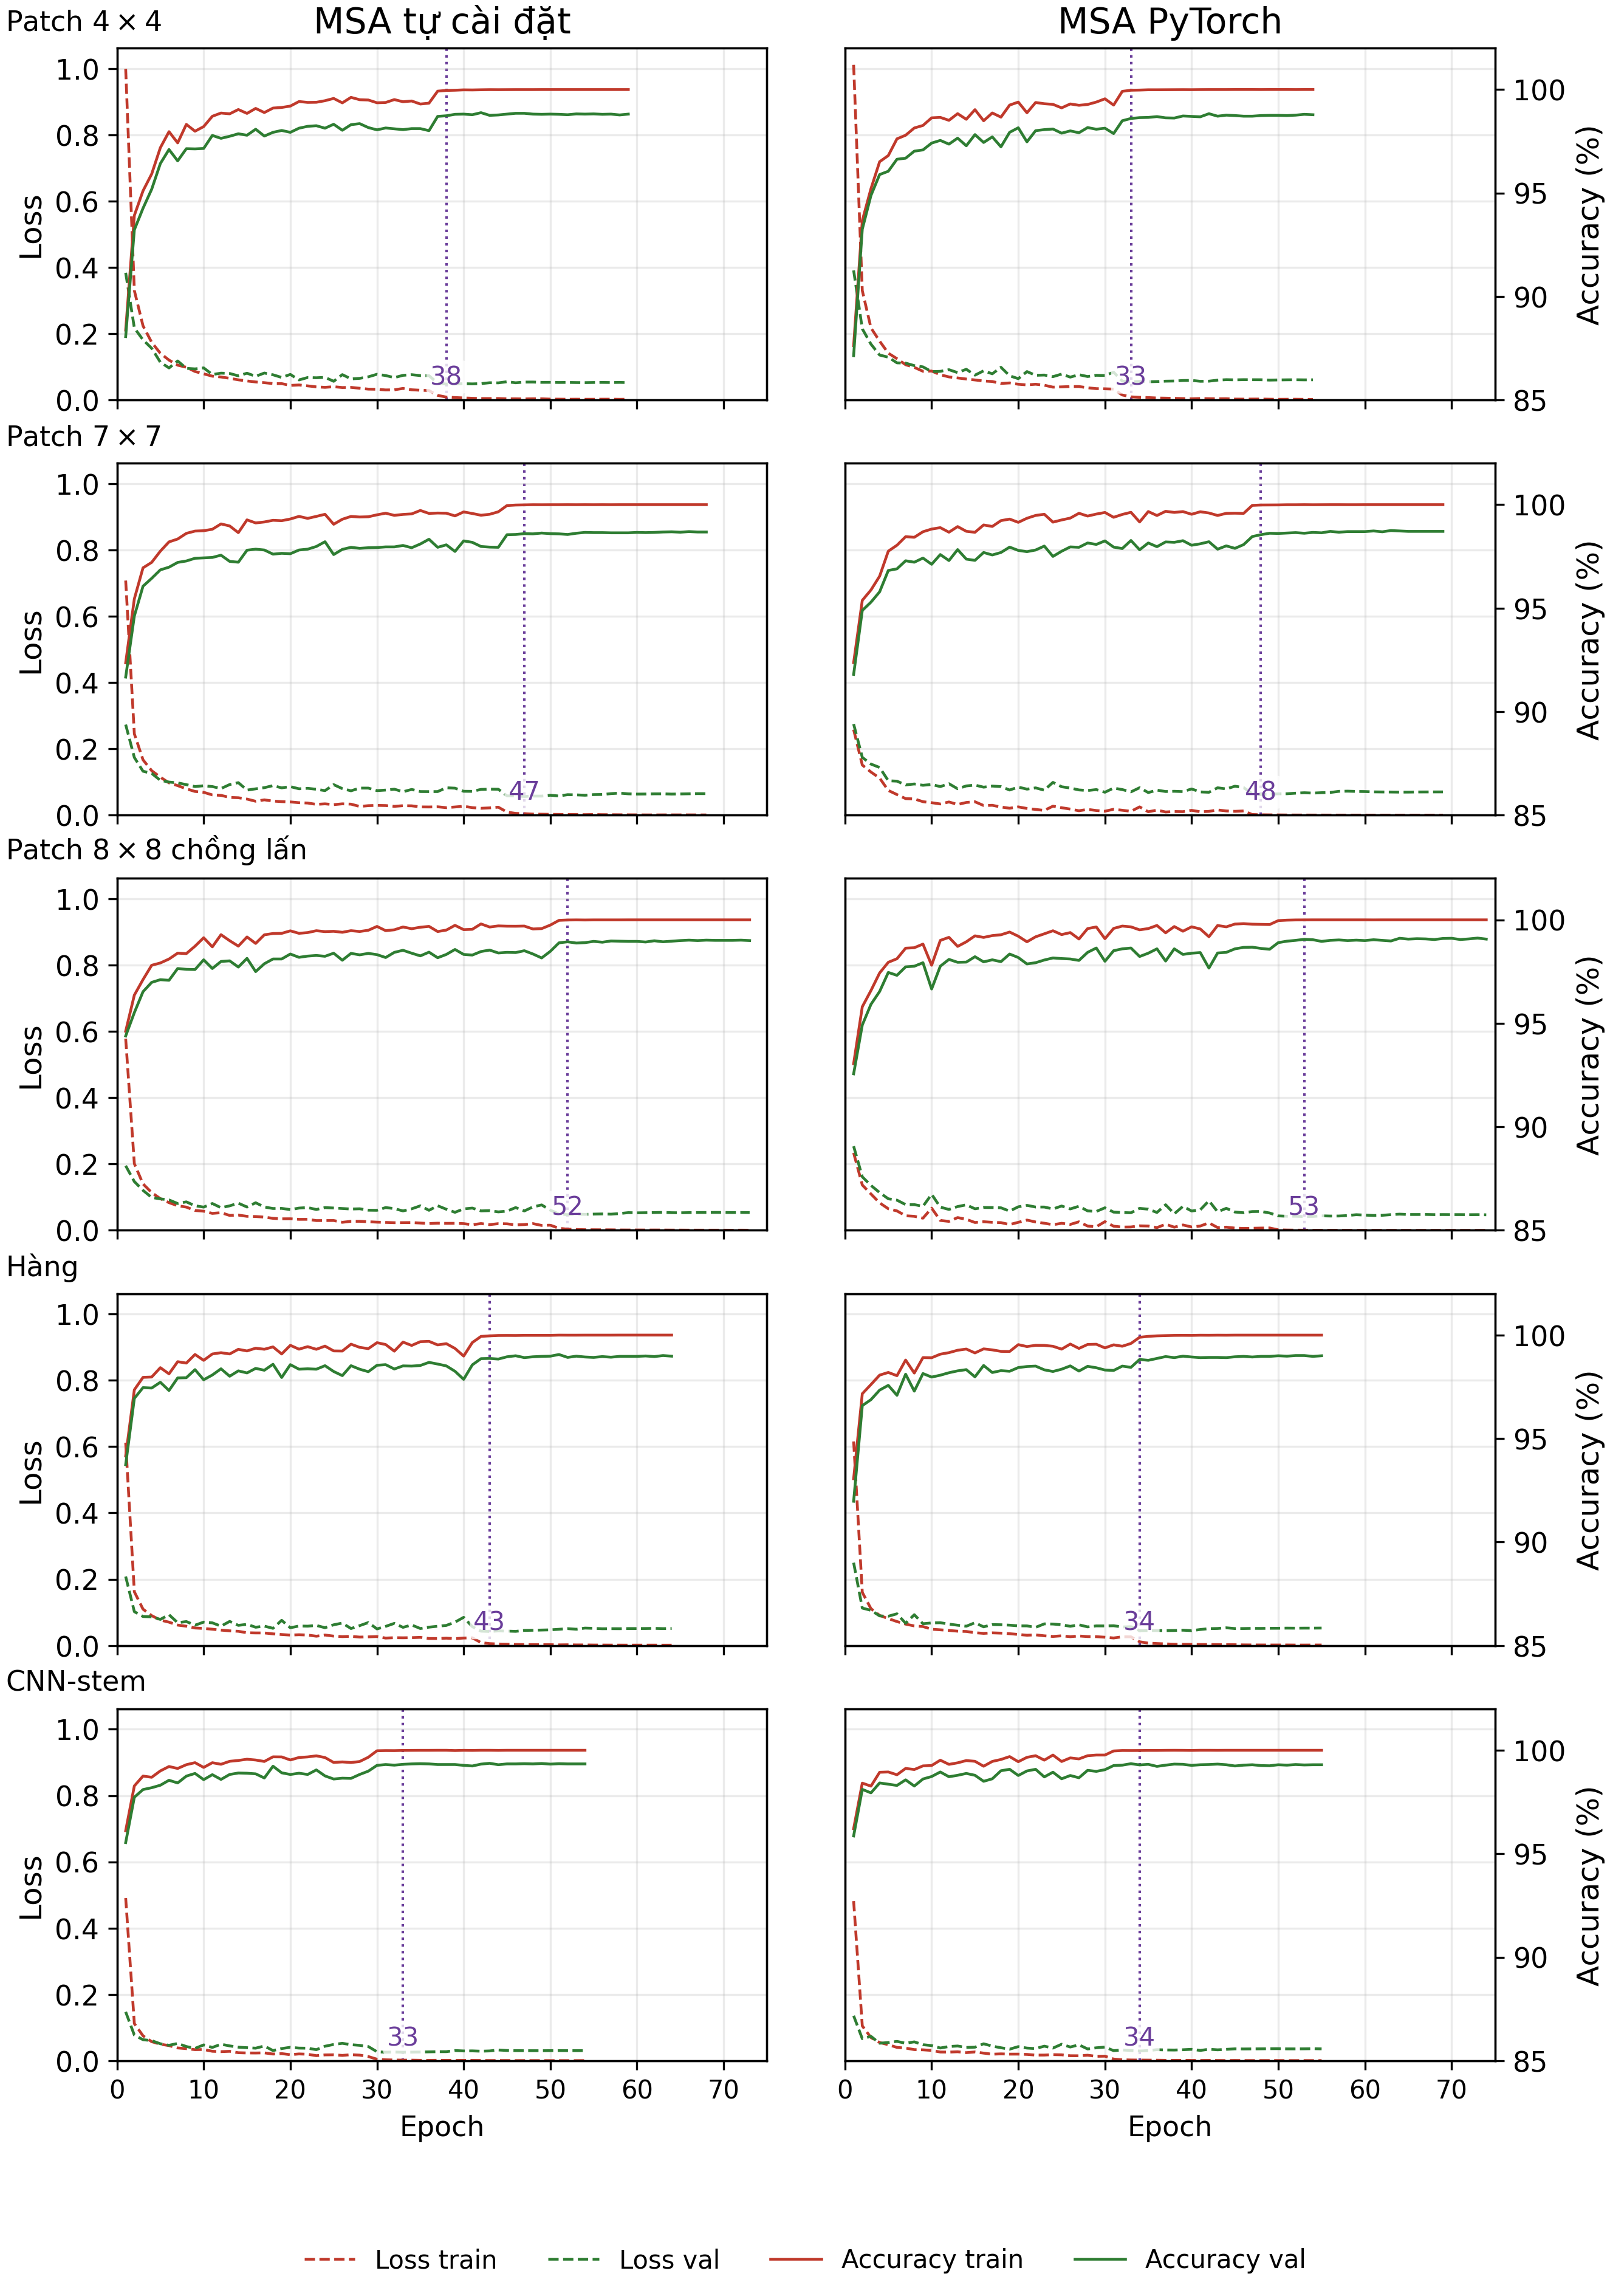
\includegraphics[width=0.8\linewidth]{../docs/assets/e2/curves_e2.png}
    \caption{Đường cong học của E2 (nét đứt: loss, trục trái; nét liền: accuracy, trục phải; đỏ: train, xanh lá: val; đường chấm tím: epoch của checkpoint được giữ). Mỗi hàng là một cách tạo token (patch $4\times4$, patch $7\times7$, patch $8\times8$ chồng lấn, hàng, CNN-stem), cột trái là MSA tự cài đặt, cột phải là MSA PyTorch. Hai bản bám sát nhau; loss val gần như phẳng sau khoảng 40 epoch trong khi accuracy train đã gần $100\%$.}
    \label{fig:e2-curves}
\end{figure}

\paragraph{Tổng số lỗi} Bảng~\ref{tab:e2-errors} thống kê số ảnh test bị phân loại sai. CNN-stem mắc ít lỗi nhất ($67$ với MSA tự cài đặt và $51$ với MSA PyTorch), trong khi patch $4\times4$ và patch $7\times7$ mắc từ $115$ đến $133$ lỗi. Hướng chênh giữa hai bản MSA không nhất quán: bản tự cài đặt mắc ít lỗi hơn ở patch $4\times4$ và hàng, nhiều lỗi hơn ở ba cách còn lại.

\begin{table}[htbp]
    \centering
    \caption{Số lượng ảnh test bị phân loại sai trên tổng số $10\,000$ mẫu.}
    \label{tab:e2-errors}
    \small
    \begin{tabular}{lrr}
        \toprule
        Cách tạo token              & MSA tự cài đặt & MSA PyTorch \\
        \midrule
        Patch $4\times4$            & 115 & 133 \\
        Patch $7\times7$            & 130 & 120 \\
        Patch $8\times8$ chồng lấn  & 102 & 93 \\
        Hàng                        & 87 & 106 \\
        CNN-stem                    & 67 & 51 \\
        \bottomrule
    \end{tabular}
\end{table}

\paragraph{Các cặp nhầm lẫn} Hình~\ref{fig:e2-confusion} cho thấy ma trận nhầm lẫn của cả mười mô hình. Cặp $4/9$ (cả hai chiều) nằm trong ba cặp bị nhầm nhiều nhất ở mọi mô hình, chẳng hạn $4\to9$ có $11$ mẫu ở patch $4\times4$ với PyTorch và $9$ mẫu ở patch $7\times7$ với MSA tự cài đặt. Cặp $5\to3$ xuất hiện ở mọi mô hình, từ $2$ mẫu (CNN-stem, PyTorch) đến $9$ mẫu (patch $7\times7$, tự cài đặt). CNN-stem mắc ít lỗi nhất nên ma trận của nó thưa nhất.

\begin{figure}[htbp]
    \centering
    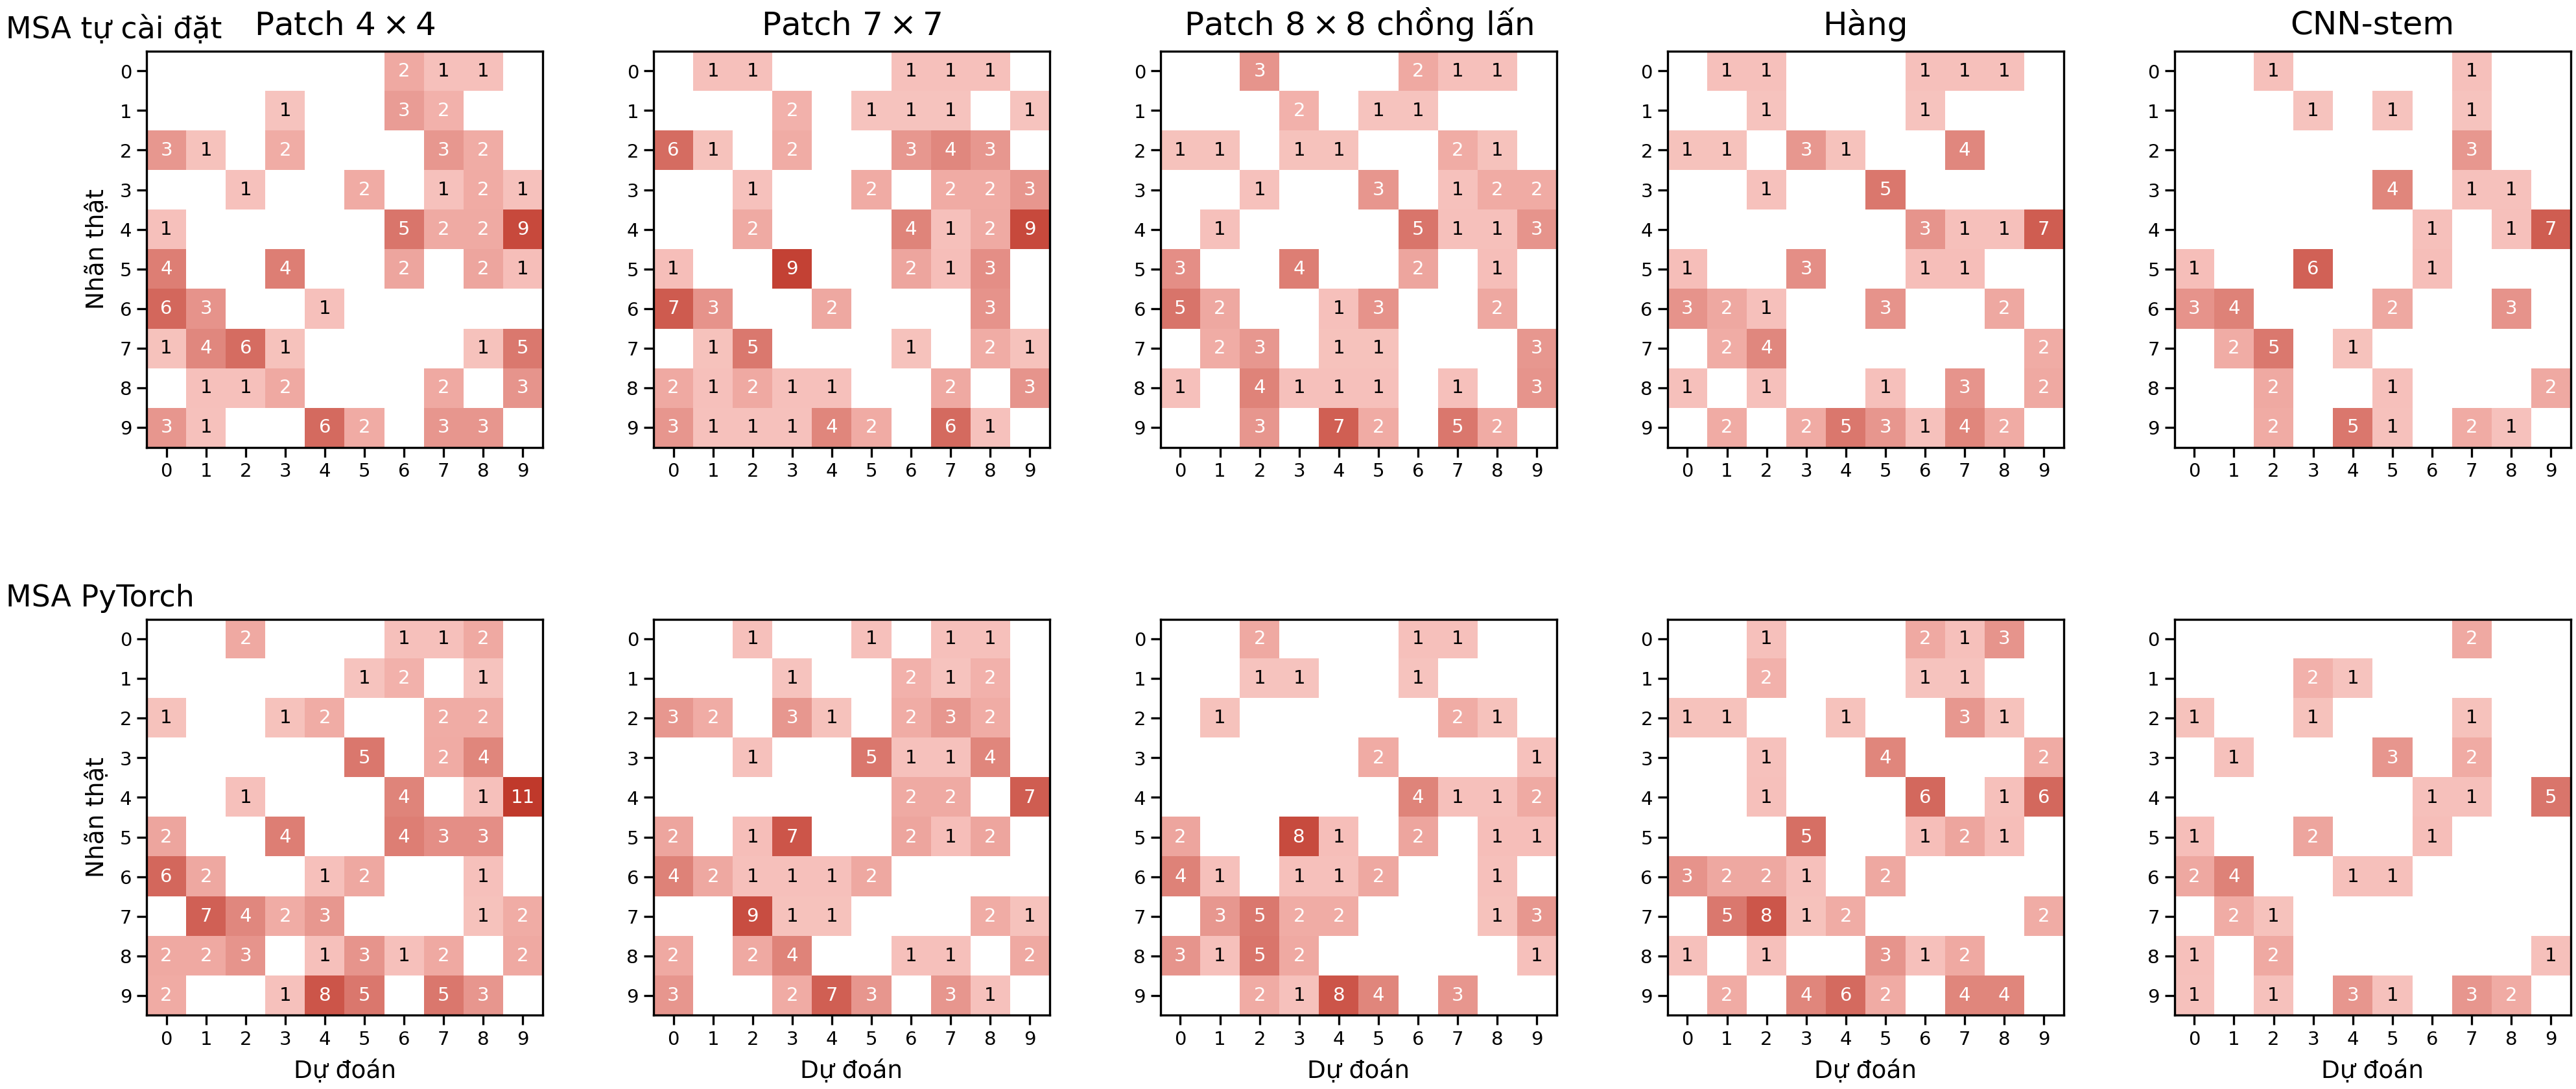
\includegraphics[width=\textwidth]{../docs/assets/e2/confusion_e2.png}
    \caption{Ma trận nhầm lẫn trên tập test của mười mô hình E2; hàng trên là MSA tự cài đặt, hàng dưới là MSA PyTorch. Ô chéo được để trắng; màu đỏ đậm hơn biểu thị tỉ lệ lỗi cao hơn; số trong mỗi ô là số mẫu bị phân loại sai.}
    \label{fig:e2-confusion}
\end{figure}

\paragraph{Mẫu bị phân loại sai} Hình~\ref{fig:e2-samples} minh họa các lỗi có độ tự tin cao nhất của CNN-stem với MSA tự cài đặt, là mô hình có accuracy val cao nhất của bài E2. Hơn một nửa trong số $20$ lỗi này thuộc các cặp chữ số vốn dễ nhầm như $4/9$, $5/3$ và $7/1$, trong đó nhiều ảnh viết khác thường, chẳng hạn một nét mảnh bị nhận thành chữ số $1$ hoặc chữ số $4$ khép kín phần đầu nên giống chữ số $9$.

\begin{figure}[htbp]
    \centering
    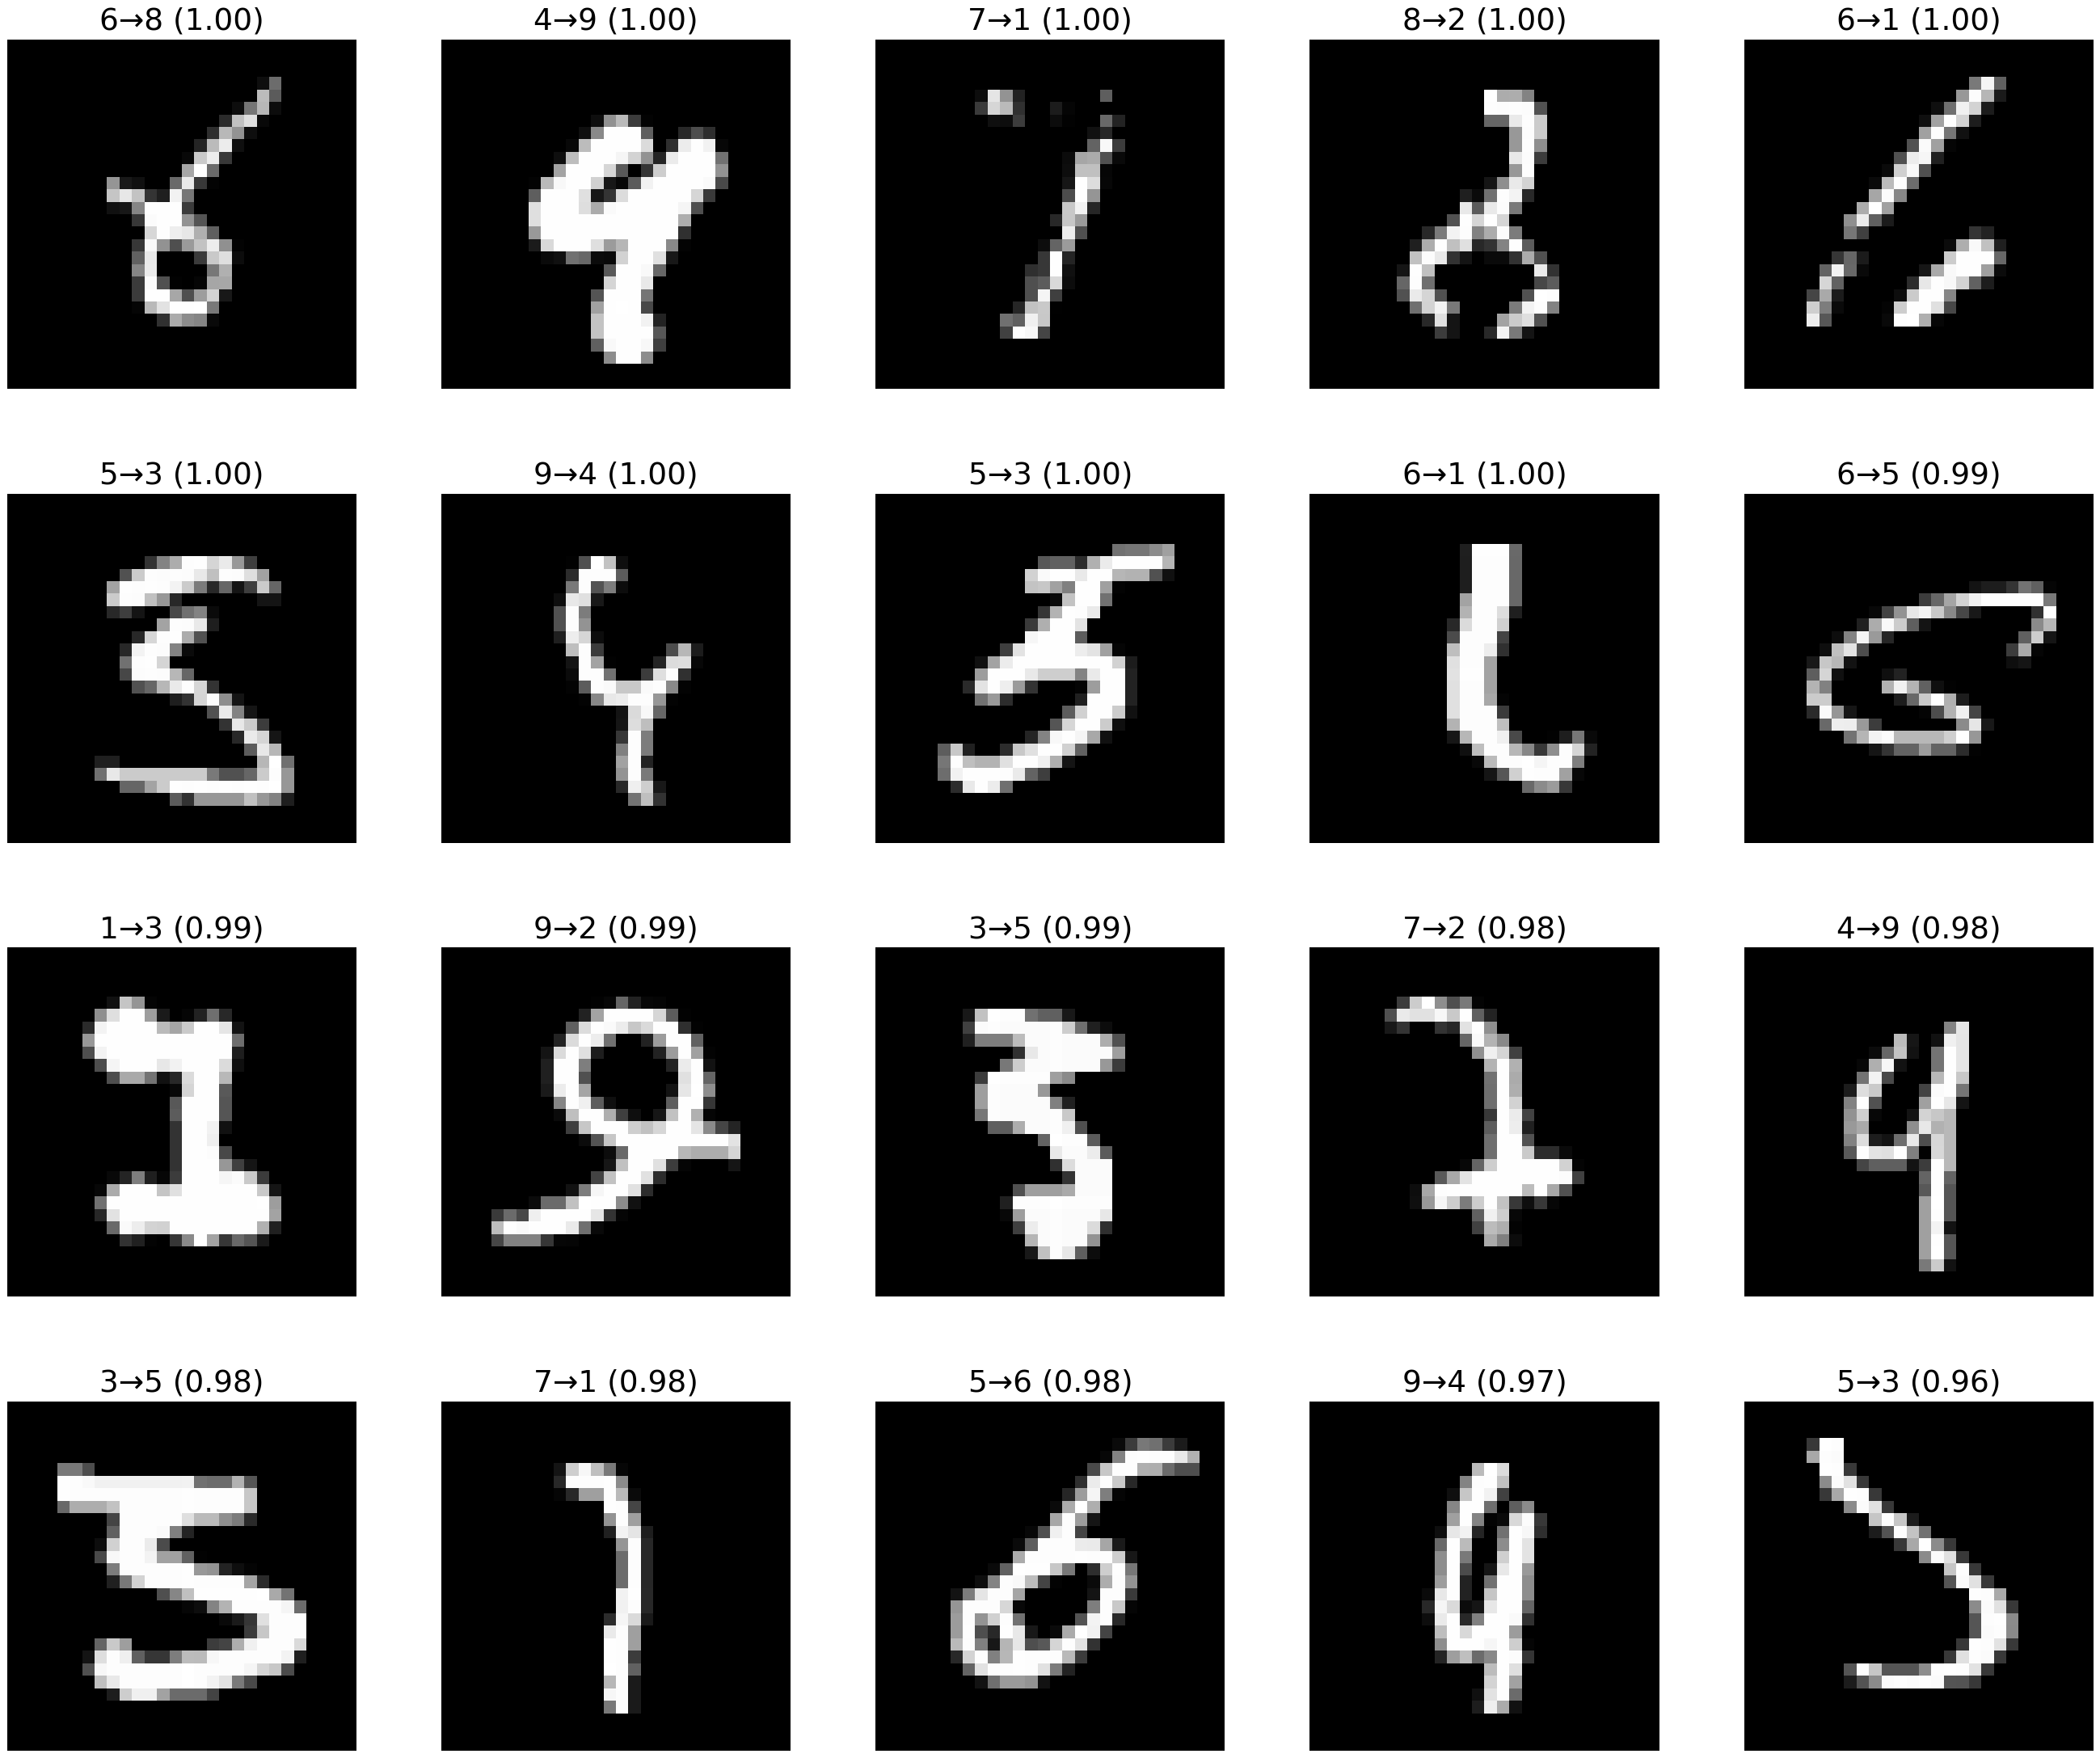
\includegraphics[width=0.85\textwidth]{../docs/assets/e2/failures_best.png}
    \caption{Một số mẫu test bị phân loại sai có độ tự tin dự đoán cao nhất của CNN-stem với MSA tự cài đặt. Mỗi ảnh ghi nhãn thật $\rightarrow$ dự đoán và xác suất của lớp dự đoán sai.}
    \label{fig:e2-samples}
\end{figure}

\subsection{Thảo luận}
\label{sec:e2-discussion}

\paragraph{Hai bản MSA tương đương} Accuracy test của hai bản gần nhau ở cả năm cách tạo token: patch $4\times4$ $98{,}85\%$ so với $98{,}67\%$, patch $7\times7$ $98{,}70\%$ so với $98{,}80\%$, patch chồng lấn $98{,}98\%$ so với $99{,}07\%$, hàng $99{,}13\%$ so với $98{,}94\%$, CNN-stem $99{,}33\%$ so với $99{,}49\%$. Chênh lệch lớn nhất là $0{,}19$ điểm và hướng chênh không nhất quán (bản tự cài đặt cao hơn ở patch $4\times4$ và hàng, thấp hơn ở patch $7\times7$, patch chồng lấn và CNN-stem), nên phù hợp với nhiễu tối ưu hơn là một khác biệt hệ thống. Vì vậy bản MSA tự cài đặt cho kết quả tương đương \texttt{nn.MultiheadAttention}. Thời gian mỗi epoch cũng không cho thấy bản nào nhanh hơn: bản tự cài đặt nhanh hơn ở patch $4\times4$ ($11{,}08$ s so với $15{,}83$ s) và patch $7\times7$ ($11{,}76$ s so với $15{,}81$ s) nhưng chậm hơn ở hàng ($16{,}03$ s so với $10{,}69$ s) và patch chồng lấn ($16{,}17$ s so với $15{,}56$ s). Con số này gồm cả thời gian nạp dữ liệu trên CPU và mỗi lượt chạy diễn ra trên một container riêng, nên nó phản ánh máy chạy nhiều hơn chi phí của mô hình; chúng tôi không dùng nó để so sánh hai cách cài đặt.

\paragraph{Cách tạo token là một dạng thiên kiến quy nạp} Với MSA tự cài đặt, accuracy test xếp từ cao xuống thấp là CNN-stem $99{,}33\%$, hàng $99{,}13\%$, patch $8\times8$ chồng lấn $98{,}98\%$, patch $4\times4$ $98{,}85\%$ và patch $7\times7$ $98{,}70\%$. CNN-stem mang thiên kiến tích chập (tính cục bộ và bất biến tịnh tiến được đưa vào trước khi attention nhìn toàn cục) và dẫn đầu, nhưng cũng có nhiều tham số nhất ($161\,098$, hơn các mô hình còn lại khoảng $16\%$), nên chưa tách được đóng góp của thiên kiến khỏi đóng góp của dung lượng. Cách tạo token theo hàng giao cho attention tự học quan hệ giữa các hàng. Với MSA tự cài đặt, hàng đạt $99{,}13\%$ trên test, cao hơn cả ba biến thể patch ($98{,}70\%$ đến $98{,}98\%$), dù xếp dưới patch chồng lấn ở accuracy val ($98{,}87\%$ so với $98{,}94\%$). Ngược lại, với MSA PyTorch, patch chồng lấn cao hơn hàng trên test ($99{,}07\%$ so với $98{,}94\%$). Chênh lệch của hàng so với patch chồng lấn ($0{,}15$ điểm) và patch $4\times4$ ($0{,}28$ điểm) dưới $0{,}3$ điểm; riêng patch $7\times7$ thấp hơn hàng $0{,}43$ điểm nhưng đây chỉ là kết quả của một seed, và thứ hạng giữa hàng với patch chồng lấn đổi chiều theo cách cài đặt MSA nên chưa ổn định. Giữa các biến thể patch của bản tự cài đặt, chênh lệch tối đa là $0{,}28$ điểm, nhỏ hơn mức dao động mà một seed duy nhất cho phép phân biệt; chúng tôi không rút ra kết luận về kích thước hay độ chồng lấn của patch.

\paragraph{Chi phí theo số token} Chi phí của attention tăng theo $O(N^2d)$ với $N$ từ $16$ (patch $7\times7$) đến $49$ (patch $4\times4$, CNN-stem). Tuy vậy thời gian mỗi epoch không tăng theo $N$ (patch $7\times7$ $11{,}76$ s, hàng $16{,}03$ s, chồng lấn $16{,}17$ s, patch $4\times4$ $11{,}08$ s) vì bị chi phối bởi việc nạp dữ liệu, nên không dùng được để kiểm chứng quan hệ $O(N^2d)$. Cột ảnh/giây trong \texttt{results\_e2.csv} đo riêng mô hình: patch $7\times7$ ($N=16$) đạt khoảng $8\,400$--$11\,000$ ảnh/s, patch $4\times4$ ($N=49$) khoảng $3\,800$--$4\,200$ và CNN-stem ($N=49$) khoảng $2\,300$--$2\,600$. Patch $7\times7$ nhanh hơn patch $4\times4$ khoảng $2{,}2$--$2{,}6$ lần, gần với tỉ lệ tuyến tính theo $N$ ($49/16\approx3{,}1$) hơn tỉ lệ bậc hai ($(49/16)^2\approx9{,}4$). Điều này phù hợp với việc ở $N\le49$ và $d=64$, phần $O(Nd^2)$ của các phép chiếu và FFN lấn át $O(N^2d)$ của attention. Kết luận này còn hạn chế: ảnh/giây được đo trên CPU của máy phân tích chứ không phải GPU lúc huấn luyện, dao động khoảng $30\%$ giữa các lần đo, và gồm cả chi phí của tokenizer (CNN-stem chậm hơn patch $4\times4$ dù cùng $N=49$).

\paragraph{So sánh với E1} E2 không tăng cường dữ liệu nên được so với các biến thể base của E1. Mọi mô hình Transformer ($98{,}67$--$99{,}49\%$) đều cao hơn MLP base ($97{,}68\%$) và có ít tham số hơn ($138\,442$--$161\,098$ so với $235\,146$). Khoảng cách khoảng $1$ đến $1{,}8$ điểm lớn hơn ngưỡng một seed. Phép so sánh này đi cùng khác biệt huấn luyện đã nêu ở phần thiết lập: E2 dùng AdamW, weight decay $0{,}05$, batch $128$, tối đa $200$ epoch; E1 dùng Adam, batch $64$, tối đa $1\,000$ epoch. Bảy trên mười mô hình ngang hoặc vượt CNN base ($98{,}85\%$, $206\,922$ tham số). CNN-stem tự cài đặt đạt $99{,}33\%$ ($67$ lỗi), cao hơn CNN base ($115$ lỗi) $0{,}48$ điểm, với ít tham số hơn ($161\,098$ so với $206\,922$); chỉ patch $4\times4$ với PyTorch ($98{,}67\%$) và patch $7\times7$ ($98{,}70\%$ và $98{,}80\%$) thấp hơn một chút. CNN-stem PyTorch đạt $99{,}49\%$ ($51$ lỗi), sát CNN có tăng cường của E1 ($99{,}50\%$, $50$ lỗi). Lệch một ảnh test, nhỏ hơn nhiều so với ngưỡng khoảng $0{,}3$ điểm, nên hai mức này chưa tách được.

\paragraph{Hạn chế} MNIST nhỏ và dễ: cả mười mô hình đều đạt trên $98{,}6\%$ với chưa tới $162\,000$ tham số, nên bài toán này khó phân biệt các cách tạo token.
\section{E3: LSTM và GRU trên chuỗi ảnh}
\label{sec:e3}
\todo{Sẽ viết sau khi có kết quả E3 (hạn nộp 09/11/2026).}

\section{So sánh tổng hợp}
\label{sec:summary}
\begin{table}[t]
    \centering
    \caption{Tất cả mô hình trên MNIST (độ chính xác kiểm tra, \%).}
    \label{tab:master}
    \small
    \begin{tabular}{llrrr}
        \toprule
        Bài & Mô hình                     & Tham số  & Test acc & Thời gian/epoch (s) \\
        \midrule
        E1  & Softmax (aug)               & 7\,850   & 85,12    & \todo{}             \\
        E1  & MLP (aug)                   & 235\,146 & 99,07    & \todo{}             \\
        E1  & CNN (aug)                   & 206\,922 & 99,50    & \todo{}             \\
        E2  & Patch $4\times4$ + MSA tự cài đặt  & 139\,018 & 98,85    & 11,08 \\
        E2  & Patch $4\times4$ + MSA PyTorch     & 139\,018 & 98,67    & 15,83 \\
        E2  & Patch $7\times7$ + MSA tự cài đặt  & 139\,018 & 98,70    & 11,76 \\
        E2  & Patch $7\times7$ + MSA PyTorch     & 139\,018 & 98,80    & 15,81 \\
        E2  & Patch $8\times8$ chồng lấn + MSA tự cài đặt & 141\,258 & 98,98    & 16,17 \\
        E2  & Patch $8\times8$ chồng lấn + MSA PyTorch & 141\,258 & 99,07    & 15,55 \\
        E2  & Hàng + MSA tự cài đặt              & 138\,442 & 99,13    & 16,03 \\
        E2  & Hàng + MSA PyTorch                 & 138\,442 & 98,94    & 10,69 \\
        E2  & CNN-stem + MSA tự cài đặt          & 161\,098 & 99,33    & 16,73 \\
        E2  & CNN-stem + MSA PyTorch             & 161\,098 & 99,49    & 15,94 \\
        E3  & \todo{LSTM/GRU tốt nhất}    & \todo{}  & \todo{}  & \todo{}             \\
        \bottomrule
    \end{tabular}
\end{table}
\todo{Thảo luận độ chính xác so với tham số so với thời gian, và thiên kiến quy nạp nào phù hợp nhất với MNIST.}

\section{Kết luận}
\begin{itemize}
    \item Kiến trúc quan trọng hơn số tham số: CNN vượt MLP dù ít tham số hơn.
    \item Tăng cường dữ liệu tương tác với dung lượng mô hình: giảm khoảng $60\%$ số lỗi của MLP và CNN nhưng làm hại softmax vì mô hình này underfitting.
    \item Tăng cường dữ liệu thay thế được một phần thiên kiến kiến trúc (MLP aug $\approx$ CNN base).
    \item Với cùng cách cài đặt MSA, CNN-stem cho accuracy test cao nhất trong năm cách tạo token ($99{,}33\%$ với MSA tự cài đặt và $99{,}49\%$ với MSA PyTorch). Bản tự cài đặt cao hơn CNN base của E1 $0{,}48$ điểm dù ít tham số hơn. Bản PyTorch lệch CNN có tăng cường một ảnh test, trong sai số của một seed. MSA tự cài đặt gần \texttt{nn.MultiheadAttention}: chênh tối đa $0{,}19$ điểm và đổi chiều giữa các cách tạo token.
    \item \todo{Kết luận E3.}
\end{itemize}
\paragraph{Hạn chế} \todo{một seed, tập dữ liệu nhỏ, tinh chỉnh hạn chế, một mức tăng cường.}

\appendix
\section{Siêu tham số chi tiết}
\todo{Bảng đầy đủ tối ưu hóa, tốc độ học, bộ lập lịch, batch size, số epoch, seed, kích thước mô hình của từng bài.}

\section{Việc sử dụng công cụ AI}
\todo{Khai báo trung thực: đã dùng công cụ AI nào, vào việc gì (ví dụ trao đổi hướng phân tích, chỉnh ngữ pháp, gợi ý soạn thảo). Theo quy định môn học, AI chỉ được dùng hỗ trợ, phải ghi rõ, và nhóm phải hiểu và bảo vệ được mã nguồn và số liệu.}

\addcontentsline{toc}{section}{Tài liệu}
\bibliographystyle{plain}
\bibliography{references}

\end{document}
